% !TEX root = ../dissertation.tex

\chapter{Mathematical Background}\label{sec:mathematical_background}
This chapeter defines and derives the mathematical models that are used throughout the reminder of this work.
Furthermore, this chapeter also provided the mathematical background in astrodynamic, geometric dynamics and control, topology, and computational geometry that are critical for the subsequent developments.
This chapter does not provide a complete treatment but rather highlights and derives the results which will be used in future chapters.

In~\cref{sec:dumbbell}, the equations of motion of a rigid dumbbell are derived in both the inertial frame and the rotating asteroid frame.
In addition, the equations of motion are each presented in the both the Lagrangian and Hamiltonian forms for a total for four separate equations of motion.
The dynamics equations of motion are crucial for the geometric controller design of~\cref{sec:se3_control} and dynamic simulations around asteroids of~\cref{sec:shape_reconstruction}.
\Cref{sec:small_body_modeling} presents the gravitational models used to represent the asteroids considered in this study. 
We summarize the spherical harmonic, constant density ellipsoid, and polyhedron potential models.
Finally,~\cref{sec:computational_geometry} presents the mathematical and computational background required to represent the wide variety of small-body shapes.
These mathematical tools and data are used throughout the thesis to efficiently determine the asteroid shape.

\section{Spacecraft Dynamic Model}\label{sec:dumbbell}

%TODO Some of these paragraphs can be moved to the introduction instead
In this section, we derive the equations of motion of a rigid spacecraft under the influence of the gravitational attraction of a homogenous asteroid.
The motion of a spacecraft around an asteroid is markedly different than that of Earth orbiting vehicles.
First, the gravitational field around an asteroid is highly irregular and complex. 
The usual assumption of a spherical potential is not valid for small or irregular shaped bodies.
Furthermore, since the magnitude of the gravitational attraction is relatively small, non-gravitational effects, such as solar radiation pressure or third-body effects, become much more significant.
As a result, the orbital environment is generally quite complex and it is difficult to generate analytical insights, such as those used in the Keplerian two-body solution.

A second key consideration is the coupling between rotational and translational states around the asteroid.
The coupling is induced due to the different gravitational forces experienced on various parts of the spacecraft.
The effect of the gravitational coupling is related to the parameter \(\epsilon = \frac{r}{R_c}\), where \(r\) is the characteristic spacecraft length and \(R_c\) is the orbital radius~\cite{hughes2004}.
For Earth based missions, the orbital radius is several orders of magnitude larger than the spacecraft length and \(\epsilon\) is small.
As a result, the corresponding gravitational moment is weak and can be neglected. 
Therefore, the translational and rotational equations of motion become decoupled and can be considered separately, significantly simplifying the analysis. 
However, for operations around an asteroid the orbital radius is much smaller, which leads to much larger values of \(\epsilon\) and much larger influence of the rotational and translational coupling.
References~\cite{elmasri2005} and~\cite{sanyal2004} investigated the coupling of an elastic dumbbell spacecraft in orbit about a central body, but only considered the case of a spherically symmetric central body.

With these insights, we seek to develop the complete coupled equations of motion of a spacecraft around an asteroid.
The equations of motion should explicitly consider the interaction of the translational and rotational dynamics.
Furthermore, the equations should be defined in a global and coordinate-free representation to allow for a single global representation of the motion of the spacecraft and asteroid.
We restrict the developments to a rigid spacecraft composed of two spherical masses connected by a massless rigid link.
This dumbbell model for a spacecraft can readily be extended to a system of particles to more faithfully represent  any arbitrary rigid body.

\subsection{Reference Frames}\label{ssec:dumbbell_eoms_reference_frames}

The first step in deriving the equations of motion is to first define the \gls{kinematics} of the spacecraft motion.
This kinematical description will be used in subsequent sections to derive the equations of motion, compute the control inputs, and simulate the motion.
There are three reference frames of interest for this problem:
\begin{enumerate}
    \item \( \gls{sym:evec}[_i] \in \R^3 \) : The standard basis vectors of the inertial reference frame.
        The inertial reference frame is assumed to be fixed with respect to the stars. 
        The origin of the frame is chosen to coincide with the center of mass of the asteroid.
        The standard inertial basis vectors are given as:
        \begin{align*}
            \evec{1} &= \begin{bmatrix} 1 & 0 & 0 \end{bmatrix}^T, \\
            \evec{2} &= \begin{bmatrix} 0 & 1 & 0 \end{bmatrix}^T, \\
            \evec{3} &= \begin{bmatrix} 0 & 0 & 1 \end{bmatrix}^T.
        \end{align*}
    \item \( \gls{sym:fvec}[_i] \in \R^3 \) : The standard basis vectors for asteroid fixed frame.
        The reference frame originates at the center of mass of the asteroid and the basis vectors are aligned with the principle motments of inertia of the asteroid.
        In addition, we assume that at the beginning of any simulation that the asteroid and inertial frames are initially aligned.
    \item \( \gls{sym:bvec}[_i] \) : The standard basis vectors for the spacecraft fixed frame.
        The frame originates at the center of mass of the spacecraft and is aligned with the principle moments of inertia of the body.
\end{enumerate}
\Cref{fig:reference_frames} shows the reference frames in use throughout this work.
\begin{figure}
    \centering
    \includegraphics[width=\textwidth]{example-image-golden}
    \caption{Representation of the three reference frames, inertial, asteroid, and spacecraft, used to describe the kinematics\label{fig:reference_frames}}
\end{figure}

With the appropriate reference frames, the configuration space of the spacecraft motion is now defined to enable the derivation of the equations of motion.
From classical mechanics, the parameters which are used to define the motion of the system are called generalized coordinates and represented by \( \vc{q} \).
The vector space defined by these coordinates is called the configuration space, \( \mathsf{Q} \), of the physical system.
Frequently, the physical parameters of the system must also satisfy some mathematical constraints, which then define a configuration manifold of all generalized coordinates within the configuration space which satisfy the constraints.
For example, the motion of a particle in three-dimensional Euclidean space can be defined by the typical generalized coordinates in the form of a vector
\begin{align*}
    \vc{r} = \begin{bmatrix}
        x_1 & x_2 & x_3
    \end{bmatrix}^T.
\end{align*}
Therefore the configuration space is then the set of all real three dimensional vectors or equivalently, \(\vc{r} \in \gls{sym:real_vector_space}[^3]\).

If we further assume that the point is constrained to the surface of a sphere, for example in the case of a spherical pendulum, then the configuration space becomes the subset of \( \R^3 \) which also define points the on sphere, \( \gls{sym:n_sphere} \).
If the particle is an extended body rather than a point mass then the orientation becomes an additional configuration parameter.
The orientation of any rigid body can be defined as the orientation of a body fixed reference frame with respect to an inertial frame. 
As a result, the configuration space for the general motion of a rigid body is defined by at a minimum of three coordinates to represent translation and three coordinates to represent the orientation.
This configuration space is the semi-direct product, \( \gls{sym:special_euclidean_group} = \R^3 \times \gls{sym:special_orthogonal_group} \), or the special euclidean group.
The special euclidean group is the group of all possible rigid body motions and defines the six degrees of freedom possible by our system.
An element of the special euclidean group can be expressed using the homogenous representation as
\begin{align*}
    \begin{bmatrix}
        R & \vc{x} \\
        0 & 1,
    \end{bmatrix}
\end{align*}
where \( R \in \SO\) is a \( 3 \times 3 \) real matrix with determinant of \( +1\) and \( \vb{x} \in \R^{3 \times 1}\) is a column vector.

% TODO Discuss the group update operation as a homogenous transformation on R^4

% TODO show example of the update operation 

In this work, we assume that the asteroid is much more massive than the spacecraft and its motion is not affected by that of the spacecraft.
This assumption allows us to treat the motion of the vehicle independently from that of the asteroid, instead of treating the more complicated full-body problem. 
In~\cref{sec:dumbbell_model}, the configuration and mass properties of the spacecraft model are explicitly defined.
Using the model, the coupled dynamics of the spacecraft are derived in the inertial frame~\cref{sec:inertial_dumbbell_eoms} and asteroid fixed frames in~\cref{sec:asteroid_dumbbell_eoms}.

\subsection{Dumbbell Spacecraft Model}\label{sec:dumbbell_model}

The dumbbell spacecraft consists of two masses connected by a massless rod and is a well-known representation of a multi body spacecraft.
Furthermore, the dumbbell model captures the important interactions of the coupling between orbital and attitude dynamics. 
As a result, this simple model is useful to capture the main characteristics of a wide variety of spacecraft configurations.
Typically, spacecraft have mass concentrated in a central structure, referred to as the bus, which houses the command and control system, actuators, fuel, sensors etc. 
In addition, comparatively light-weight solar panels extend from the bus to provide electrical energy from solar radiation. 
As a result, the distributed mass of the spacecraft is captured with the dumbbell representation.

The dumbbell is defined by two spherical masses of radius \( \radius{1}, \radius{2} \in \R \) with masses \( \mass{1}, \mass{2} \in  \R\).
The masses are seperated by a massless rod of length \( \length{} \) and attached to the centers of each mass.
\Cref{fig:dumbbell_sc} shows the model and associated parameters.
\begin{figure}[htbp]
    \centering
    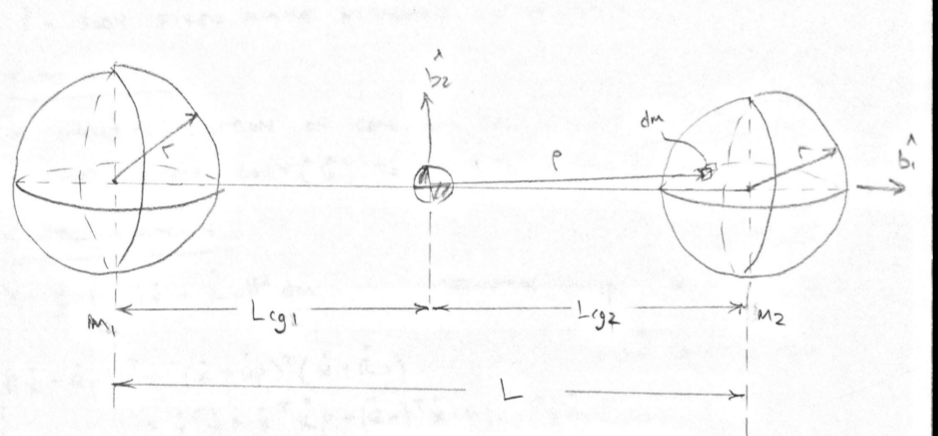
\includegraphics[width=\textwidth]{figures/dumbbell.png}
    \caption{Dumbbell Model of Rigid Spacecraft}
    \label{fig:dumbbell_sc}
\end{figure}
The spacecraft body fixed frame is centered at the center of mass of the vehicle.
The \( \bvec{1} \)  axis is aligned with the connecting rod and directed along the axis of symmetry.
The \( \bvec{2}, \bvec{3} \) axes span the plane orthogonal to the axis of symmetry of the dumbbell.
The distance from the center of mass to each spherical mass is defined as
\begin{align}\label{eq:dumbbell_mass_distances}
    \length{1} &= \frac{\mass{2}}{\mass{1} + \mass{2}} \length{}, \\
    \length{2} &= \length{} - \length{1}.
\end{align}

\paragraph{Moment of Inertia Derivation}\label{sec:moment_of_inertia}
The inertia tensor/matrix of a rigid body is defined~\cite{greenwood1988} as
\begin{align}\label{eq:moi_definition}
    J_I = \int_{\mathcal{B}} \bracket{ \parenth{\brho{}^T \brho{} }I - \brho{}\brho{}^T} dm, 
\end{align}
where \( \vb{\rho} \in \R^3 \) is the position of a mass element \( dm \) in the body fixed frame of the spacecraft.
One can also use~\cref{eq:xTx} to define the inertia matrix in several other equivalent forms
\begin{align*}
    J_I &= \int_{\mathcal{B}} \bracket{ \parenth{\vc{\rho}^T \vc{\rho} }I - \vc{\rho}\vc{\rho}^T} dm, \\
        &= \int_{\mathcal{B}} \tr{\vc{\rho}\vc{\rho}^T} I - \vc{\rho}\vc{\rho}^T, \\
        &= \int_{\mathcal{B}} \vh{\rho}^T \vh{\rho} dm.
\end{align*}
The location of an infinitesimal mass element \( dm \) can be decomposed into
\begin{align}\label{eq:mass_element_position}
    \vc{\rho}_i = \vc{\zeta} + \vc{\eta}_i, 
\end{align}
where \( \vc{\zeta} \) is the location of the center of \( m_i \) in the spacecraft fixed frame while \( \vc{\eta} \) the position of \( dm \) with respect to the center of \( m_i \) and expressed in the spacecraft fixed frame.
\begin{figure}[htbp]
    \centering
    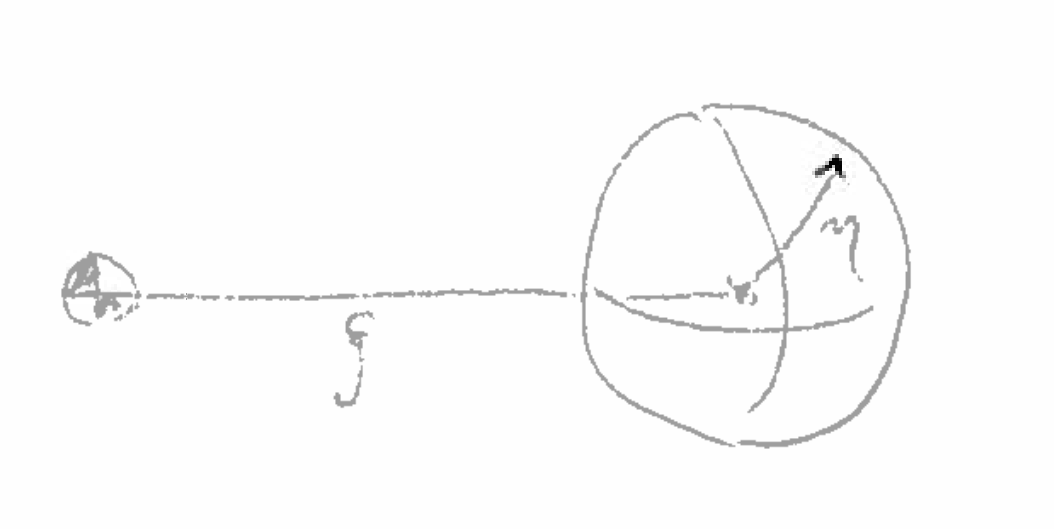
\includegraphics[width=\textwidth]{figures/dumbbell_pos_vector.png}
    \caption{Decomposition of mass element positon vector}
    \label{fig:dumbbell_moi_mass_element_position}
\end{figure}
Using~\cref{eq:mass_element_position}, the moment of inertia can be expanded as
\begin{align*}
    J_I &= \sum_i^n \int_{\mathcal{B}_i} \parenth{\vc{\zeta}_i + \vc{\eta}_i}^T \parenth{\vc{\zeta}_i + \vc{\eta}_i } I  - \parenth{\vc{\zeta}_i + \vc{\eta}_i} \parenth{\vc{\zeta}_i + \vc{\eta}_i}^T dm .
\end{align*}
Further expansion leads to
\begin{align*}
    J_I = \sum_i^n \int_{\mathcal{B}_i} \parenth{\vc{\zeta}_i^T \vc{\zeta}_i}I - \vc{\zeta}_i \vc{\zeta}_i^T + \vc{\eta}_i^T \vc{\eta}_i I - \vc{\eta}_i \vc{\eta}_i^T dm.
\end{align*}
Since the cross terms include an integration over the constant density sphere, the terms of the form
\begin{align*}
    \int_{\mathcal{B}_i} \vc{\eta}_i dm = 0,
\end{align*}
all become zero.
The integration is now split into two components: an integration within each sphere consisting of \( \vc{\eta}_i \) terms and an integration involving the location of the sphere in the spacecraft fixed frame consisting of \( \vc{\zeta}_i \) terms.
As a result, the final moment of inertia of a system of rigid spherical masses is 
\begin{align}\label{eq:dumbbell_moment_of_inertia}
    J_I = \sum_i^n J_i + m_i \parenth{\vc{\zeta}_i^T \vc{\zeta}_i I - \vc{\zeta}_i \vc{\zeta}_i^T} , 
\end{align}
where \( \vc{\zeta}_i \) is the position of \( m_i \) in the spacecraft fixed frame and the moment of inertia of each sphere is
\begin{align}\label{eq:sphere_moment_of_inertia}
    J_i = \begin{bmatrix} 
        \frac{2}{5} m_i r_i^2 & 0 & 0 \\
        0 & \frac{2}{5} m_i r_i^2 & 0 \\
        0 & 0 & \frac{2}{5} m_i r_i^2 
    \end{bmatrix}.
\end{align}
\Cref{eq:dumbbell_moment_of_inertia} is consistent with the well-known parallel-axis theorem~\cite{greenwood1988}.

%TODO Nonstandard moment of inertia matrix
\paragraph{Nonstandard Moment of Inertia Matrix}\label{sec:nonstandard_moi}
The standard moment of inertia \( J \in \R^{3 \times 3} \) of a rigid body is given by
\begin{align}\label{eq:standard_moment_of_inertia}
    J = \int_{\mathcal{B}} \vh{\rho}^T \vh{\rho} dm 
    = \int_{\mathcal{B}}  
    \begin{bmatrix} 
        y^2 + z^2 & -xy & -zx \\
        -xy & z^2 + x^2 & -yz \\
        -zx & yz & x^2 + y^2
    \end{bmatrix} dm, 
\end{align}
where \( \vc{\rho} = \begin{bmatrix} x & y & z \end{bmatrix}^T\).
A nonstandard moment of inertia matrix \( J_d \in \R^{3 \times 3 } \) is defined as
\begin{align} \label{eq:nonstandard_moment_of_inertia}
    J_d = \int_{\mathcal{B}} \vc{\rho} \vc{\rho}^T dm = \int_{\mathcal{B}} 
    \begin{bmatrix}
        x^2 & xy & zx \\
        xy & y^2 & yz \\
        zx & yz & z^2
    \end{bmatrix} dm.
\end{align}
Using~\cref{eq:xTx} and the properties of the outer product, it can be shown that
\begin{subequations}\label{eq:moi_transformation}
    \begin{align}
        J &= \tr{J_d} I - J_d, \label{eq:moi_ns2s}\\
        J_d &= \frac{1}{2} \tr{J} I - J.\label{eq:moi_s2ns}
    \end{align}
\end{subequations}     
In addition, the following equation is also satisfied for any \( \vc{\Omega} \in \R^3 \)
\begin{align}\label{eq:moi_hat_prop}
    \parenth{J \vc{\Omega}}^\wedge = \vh{\Omega} J_d + J_d \vh{\Omega}.
\end{align}
\Cref{eq:moi_hat_prop} is easy to prove by substituting \( \vc{\Omega} = \begin{bmatrix} \Omega_1 & \Omega_2 & \Omega_3 \end{bmatrix}^T \) and expanding both sides of~\cref{eq:moi_hat_prop} to
\begin{align*}
    \begin{bmatrix}
        \parenth{J_{yy} + J_{zz}} \Omega_1 - J_{xy} \Omega_2 - J_{zx} \Omega_3 \\
        -J_{xy}\Omega_1 + \parenth{J_{zz} + J_{xx}} \Omega_2 - J_{yz}\Omega_3 \\
        -J_{zx}\Omega_1 - J_{yz}\Omega_2 + \parenth{J_{xx} + J_{yy}} \Omega_3
    \end{bmatrix}^\wedge,
\end{align*}
where \( J_{xy} = \int_{\mathcal{B}} xy dm \in \R \) and the other terms are defined similarly.

\subsection{Inertial Frame Equations of Motion}\label{sec:inertial_dumbbell_eoms}
By expressing the motion of the spacecraft directly on the special euclidean group, we avoid the issues inherent in using other kinematic representations.
It has been shown the all attitude parameterizations fail to preserve the geometric properties of the configuration space~\cite{chaturvedi2011a}.
The kinematics of the spacecraft and asteroid are described in the inertial frame by
\begin{itemize}
    \item \( \gls{sym:ipos} \in \R^3 \): the position of the center of mass of the spacecraft represented in the inertial frame \( \evec{i} \),
    \item \( \gls{sym:iatt} \in \SO\): the rotation matrix which transforms vectors defined in the spacecraft fixed frame, \( \bvec{i} \), to the inertial frame, \( \evec{i} \)
    \item \( \gls{sym:iangvel} \in \R^3 \): the angular velocity of the spacecraft body fixed frame relative to the inertial frame and represented in the spacecraft body fixed frame \( \bvec{i} \)
    \item \( \gls{sym:aatt} \in \SO \): the rotation matrix which transforms vectors defined in the asteroid fixed frame, \( \fvec{i} \), to the inertial frame, \( \vecbf{e}_i \)
\end{itemize}

The motion of a rigid body spacecraft under the influence of gravity can be described by Lagrangian and Hamiltonian dynamics.
The Lagrangian function \( L : \T \Q^n \to \R^1 \) is a function of the configuration variables and their time derivatives.
The Lagrangian is defined as the system kinetic energy minus the system potential energy.
As a result, we derive the we first derive the kinetic and potential energy of the spacecraft, then apply the calculus of variations to determine the equations of motion.

\paragraph{Kinetic Energy of Dumbbell}\label{sec:inertial_kinetic_energy}
The kinetic energy of the spacecraft begins with the kinematics defined in~\cref{ssec:dumbbell_eoms_reference_frames} as
\begin{align}\label{eq:inertial_KE_1}
    T = \frac{1}{2} \int_{\mathcal{B}} \norm{ \dot{\vc{x}} + \dot{R} \vc{\rho}}^2 dm,
\end{align}
where \( \vc{\rho} \in \R^3 \) defines the position of the mass element \( dm \) in the body fixed frame of the spacecraft.
Expanding the quadratic term in~\cref{eq:inertial_KE_1} results in
\begin{align}\label{eq:inertial_KE_2}
T = \frac{1}{2} \int_{\mathcal{B}}  \norm{\dot{\vc{x}}}^2 + 2 \dot{\vc{x}}^T \dot{R} \vc{\rho} + \norm{\dot{R} \vc{\rho} }^2    dm .
\end{align}
\Cref{eq:inertial_KE_2} is further simplified by noting that
\begin{align*}
    \int_{\mathcal{B}} \vc{\rho} dm = 0,
\end{align*}
and from using the attitude kinematics \( \dot{R} = \iatt \vh{\Omega} \) for \( \vc{\Omega} \in \R^3 \) 
\begin{align*}
    \norm{\dot{R} \vc{\rho} }^2 &= \vc{\rho}\dot{R}^T \dot{R} \vc{\rho} , \\
                                &=  \vc{\rho}^T \vh{\Omega}^T \vh{\Omega} \vc{\rho} , \\
                                &= \norm{ \vh{\Omega} \vc{\rho} }^2, 
\end{align*}
which results in the following expression for the kinetic energy
\begin{align}\label{eq:inertial_KE_3}
    T = \frac{1}{2} \int_{\mathcal{B}} \braces{ \norm{\dot{\vc{x}}}^2 + \norm{\vh{\Omega} \vc{\rho}}^2 } dm.
\end{align}
The second term \( \norm{\vh{\Omega}\vc{\rho}}^2 \) is simplified to
\begin{align}
    \norm{ \vh{\Omega}\vc{\rho} }^2 &= \parenth{ \vh{\Omega}\vc{\rho}}^T \parenth{\vh{\Omega}\vc{\rho}} , \nonumber\\
                                    &= \tr{ \vh{\Omega} \vc{\rho} \vc{\rho}^T \vh{\Omega}^T }.\label{eq:omegarhosquared}
\end{align}
Applying~\cref{eq:omegarhosquared} to~\cref{eq:inertial_KE_3} results in the final form of the kinetic energy as
\begin{align}\label{eq:inertial_kinetic_energy}
    T = \frac{1}{2} m \norm{\dot{\vc{x}}}^2 + \frac{1}{2} \tr{ \vh{\Omega}J_d \vh{\Omega^T } }, 
\end{align}
where we applied the non-standard moment of inertia defined in~\cref{eq:nonstandard_moment_of_inertia}.

\paragraph{Potential Energy of Dumbbell}
The potential energy of the dumbbell is a function of the asteroid potential model.
There are a number of possible models as shown in~\cref{sec:gravitational_models}.
For a rigid body composed of several spherical point masses, the total potential is defined as
\begin{align}\label{eq:inertial_potential_energy}
    V(\vc{x}, R, R_A) = \sum_{i}^n - m_i U \parenth{R_A^T \parenth{\vc{x} + R \vc{\rho}_i}},
\end{align}
where \( \vc{x} \in \R^3\) is the position of the center of mass, \( R \in \SO\) is the rotation matrix which transforms vectors from the spacecraft frame to the inertial frame, and \( R_A \in \SO \) is the rotation matrix which transforms vectors from the asteroid frame to the inertial frame.
The exterior gravitational potential of the body is defined by \( U \in \R^1 \).

Using our kinematic variables we can define the kinetic and potential energy of the dumbbell using~\cref{eq:inertial_kinetic_energy,eq:inertial_potential_energy} as
\begin{subequations}\label{eq:dumbbell_kinetic_and_potential_energy}
\begin{align}
    T &= \frac{1}{2} m \norm{\dot{\vc{x}}}^2 + \frac{1}{2} \tr{\vh{\Omega} J_d \vh{\Omega}^T} , \label{eq:dumbbell_kinetic_energy}\\
    V( \vecbf{x}, R ) &=  - m_1 U \parenth{R_A^T \parenth{\vc{x} + R \vc{\rho}_1}} - m_2 U \parenth{R_A^T \parenth{\vc{x} + R \vc{\rho}_2}}. \label{eq:dumbbell_potential_energy}
\end{align}
\end{subequations}     
In this work we will utilize the polyhedron potential model defined in~\cref{sec:polyhedron_potential}.
The position of each mass \(m_i\) of the dumbbell is defined in the dumbbell fixed frame by the vector \(\vc{\rho}_i\). 
With~\cref{eq:dumbbell_kinetic_and_potential_energy} one can then use Hamilton's principle  and the variation of the action integral to derive the equations of motion.
However, the first step is to determine the variation of the kinetic and potential energies.
These variations must be carefully constructed such that the variations of the configuration variables do not violate the geometric properties of the configuration space.
The variations of~\cref{eq:dumbbell_kinetic_and_potential_energy} are given by
\begin{align} 
    \delta T &= \parenth{m_1 + m_2} \ivel^T \delta \dot{\ipos} + \frac{1}{2} \tr{- \dot{\iattvar} \parenth{J \iangvel}^\wedge + \iattvar \parenth{\hat{\iangvel} J \iangvel}^\wedge }, \label{eq:dumbbell_kinetic_energy_variation} \\
    \delta V &= - \sum_{i=1}^2 \braces{ \bracket{m_i \deriv{U}{\apos_i}^T \aatt^T } \delta \ipos +  \tr{\iattvar \parenth{\spos_i \deriv{U}{\apos_i}^T \aatt^T \iatt } }},\label{eq:dumbbell_potential_energy_variation}
\end{align}
where \( \apos_i = \aatt^T \parenth{\ipos + \iatt \spos_i} \) defines the position of \( m_i \) in the asteroid fixed frame.
The detailed derivation of~\cref{eq:dumbbell_potential_energy_variation,eq:dumbbell_kinetic_energy_variation} is provided in~\cref{proof:inertial_dumbbell_eoms}.

Using the variation of the Lagrangian, we can derive the equations of motion of the dumbbell spacecraft about an asteroid using Hamilton's principle. 
Hamilton's principle states that the variation of the action integral
\begin{align}\label{eq:action_integral}
    \mathcal{G} = \int_{t_0}^{t_f} T(\dot{\vc{q}}) - V(\vc{q}) dt,
\end{align}
is stationary for all possible variations with fixed endpoints. 
In other words, 
\begin{align}\label{eq:hamiltons_principle}
    \delta \mathcal{G}  = \int_{t_0}^{t_f} \delta T - \delta V dt = 0.
\end{align}
The detailed derivation is presented in~\cref{proof:inertial_dumbbell_eoms}.
The inertial equations of motion can be written in Lagrangian form as
\begin{align}
    \dot{\ipos} &= \ivel, \label{eq:inertial_position_dynamics}\\
    \parenth{m_1 + m_2} \dot{\ivel} &= - \sum_{i=0}^2 m_i \aatt \deriv{U}{\apos_i} + u_f, \label{eq:inertial_velocity_dynamics}\\
    \dot{\iatt} &= \iatt \iangvel, \label{eq:inertial_attitude_dynamics}\\
    J \dot{\iangvel} + \hat{\iangvel} J \iangvel &= \sum_{i=0}^2 m_i \hat{\spos}_i \iatt^T \aatt \deriv{U}{\apos_i} + u_m. \label{eq:inertial_angvel_dynamics}
\end{align}
The vectors \( \apos_i \) define the position of the dumbbell mass \( m_i \) in the asteroid fixed frame
\begin{align}\label{eq:mass_asteroid_frame}
    \apos_i &= \aatt^T \parenth{\ipos + \iatt \spos_i},
\end{align}
where \( \spos_i \) defines the position of each mass in the spacecraft fixed body frame.
The control inputs to the spacecraft are defined by \( u_f, u_m \in \R^3 \) which define the control force represented in the inertial frame and the control moment represented in the spacecraft frame, respectively. 

\paragraph{Inertial Equations of motion: Hamiltonian Form}\label{sec:inertial_hamiltonian_form}
% TODO Check hte legendre transformation is correct
Hamilton's equations allows for the representation of the second order equations derived using the Euler-Lagrange equation as a system of \( 2n \) first order equations called a hamiltonian system of equations or canonical equations~\cite{arnold1989}.
Hamilton's equations are derivable direclty from the Lagrangian through the use of the Legendre transformation which is a mapping \( \left( q, \dot{q},t\right) \rightarrow \left(q, p, t \right) \) where \( p_i\) is the generalized momenta,
\begin{align}\label{eq:legendre_transform}
	p_i = \deriv{L}{\dot{q}}
\end{align}
The Legendre transformation is useful for variational equations of the form
\begin{align*}
	df &= u dx + v dy, \\
	u &= \deriv{f}{x},\quad v = \deriv{f}{y}.
\end{align*}
To change from \( \left( x, y\right) \rightarrow \left(u,y \right) \) on can use the transformation
\begin{align*}
	g &= f - u x,\\
	dg &= df - u dx - x du, \\
	dg &= v dy - x du, \\
	x&= -\deriv{g}{u}, \\
    v&= \deriv{g}{y}.
\end{align*}

In the continuous time case, one can define the Hamiltonian in terms of the Lagrangian as
\begin{align}\label{eq:hamiltonian}
	H &= \sum_{i = 1}^N p_i \dot{q}_i - L \left( q_i,\dot{q}_i, t \right)
\end{align}
Applying~\cref{eq:legendre_transform} and taking the variation of~\cref{eq:hamiltonian} allows us to derive the equations of motion in Hamiltonian form as
\begin{align}\label{eq:hamilton_eq}
	\dot{q}_i &= \deriv{H}{p_i}, \\
	\dot{p}_i &= - \deriv{H}{q_i} + Q_i, \\
	\deriv{L}{t} &= -\deriv{H}{t}.
\end{align}
Again we are left with \( 2n \) first order differential equations that describe the system dynamics in terms of the generalized position and momenta \( q_i \) and \( p_i\), respectively.
For the inertial equations of motion, we define the linear and angular momentum of the spacecraft as \( \gls{sym:ilinmom} \in \R^3\) and \( \gls{sym:iangmom} \in \R^3 \), respectively.
The system momenta are related to the velocities by the transformations
\begin{align}
    \ilinmom &= \parenth{m_1 + m_2} \ivel , \\
    \iangmom & = J \iangvel.
\end{align}
The continuous inerital equations of motion in Hamiltonian form are defined as
\begin{align}
    \dot \ipos &= \frac{\ilinmom}{m_1 + m_2}, \label{eq:inertial_position_dynamics_hamiltonian}\\
    \dot \ilinmom &= - m_1 \aatt \deriv{U}{\apos_1} - m_2 \aatt \deriv{U}{\apos_2}, \label{eq:inertial_velocity_dynamics_hamiltonian}\\
    \dot \iatt &= R \parenth{J^{-1} \iangmom}^\wedge, \label{eq:inertial_attitude_dynamics_hamiltonian}\\
    \dot\iangmom  + \hat{\iangvel} \iangmom &= m_1 \hat{\spos}_1 \iatt^T \aatt \deriv{U}{\apos_1} + m_2 \hat{\spos}_2 \iatt^T \aatt \deriv{U}{\apos_2}. \label{eq:inertial_angvel_dynamics_hamiltonian}
\end{align}

\subsection{Asteroid Frame Equations of Motion}\label{sec:asteroid_dumbbell_eoms}
The complete motion of rigid bodies under the influence of their mutual gravity only depends on the relative position and relative attitude of the bodies~\cite{lee2007a}.
This is a consequence of the fact that the gravitational potential can be described using only the relative position.
Physically, this is due to the fact that the total linear and angular momentum of the system is conserved.
In astrodynamics, this fact is typically used to reduce the two body problem to that of the relative two body problem which affords convienent analytical solutions~\cite{vallado2007,bate1971}.
In this section, the equations of motion of a rigid spacecraft are derived in the asteroid fixed frame.
This derivation can be considered a specific example of the relative full body problem and is readily generalized to multiple bodies~\cite{lee2007a}.

The relative motion of a dumbbell spacecraft with respect to an asteroid are defined by the kinematics:
\begin{align}
    \gls{sym:rpos} &= R_A^T \vc{x}, \label{eq:relative_position} \\
    \gls{sym:rvel} &= R_A^T \dot{\vc{x}}, \label{eq:relative_velocity},
\end{align}
where \( \rpos \in \R^3 \) is the relative position of the spacecraft with respect to the asteroid and expressed in the asteroid fixed frame, and \( \rvel \in \R^3 \) is the relative velocity of the spacecraft with respect to the asteroid and expressed in the asteroid fixed frame.
The relative attitude kinematics are defined by
\begin{align}
    \gls{sym:ratt} &= R_A^T R, \label{eq:relative_attitude} \\
    \gls{sym:rangvel} &= \ratt  \vc{\Omega}, \label{eq:relative_angular_velocity}
\end{align}
where \( \ratt \in \SO \) is the relative attitude of the spacecraft with respect to the asteroid.
\( \ratt \) transforms vectors from the spacecraft fixed frame to the asteroid fixed frame.
\( \rangvel \in \R^3 \) is the angular velocity of the spacecraft with respect to the inertial frame and expressed in the asteroid frame.

As in~\cref{sec:inertial_dumbbell_eoms}, we first seek to define the kinetic and potential energy of the dumbbell in terms of these relative kinematics. 
Afterwards, the variations are taken to derive the equations of motion.
In this analysis, it is assumed that the motion of the asteroid is not impacted by that of the dumbbell.
In other words, the size of the dumbbell spacecraft is significantly less than that of the asteroid. 
As a result, the motion of the asteroid is unaffected by that of the spacecraft.

The kinetic energy defined in the inertial frame is given by~\cref{eq:inertial_kinetic_energy} and is transformed using~\cref{eq:relative_position,eq:relative_angular_velocity} as
\begin{align}\label{eq:relative_kinetic_energy_1}
    T &= \frac{1}{2} \parenth{m_1 + m_2} \parenth{\rvel \aatt^T \aatt \rvel} + \frac{1}{2} \tr{\parenth{\ratt^T \rangvel}^\wedge J_d \parenth{\ratt^T \rangvel }^{\wedge T}}. 
\end{align}
Using~\cref{eq:hatRxR,eq:trABC} in~\cref{eq:relative_kinetic_energy_1} results in
\begin{align}\label{eq:relative_kinetic_energy_2}
    T = \frac{1}{2} \parenth{m_1 + m_2} \norm{\rvel}^2 + \frac{1}{2} \tr{\rhangvel \ratt J_d \ratt^T \rhangvel^T}.
\end{align}
The term \( \ratt \Jdi \ratt^T = \Jdr\) is the expression of the nonstandard moment of inertia tensor of the dumbbell expressed in the asteroid fixed frame. 
It is now a time varying inertia matrix as the relative attitude \( \ratt \) is a function of time.
Using~\cref{eq:hatRxR} it can be shown that \( \Jdr \) also satisfies a similar property as~\cref{eq:moi_hat_prop}, 
\begin{align}\label{eq:moi_relative_hat_prop}
    \parenth{\Jr \rangvel}^\wedge = \rhangvel \Jdr + \Jdr\rhangvel,
\end{align}
where \( \Jr = \ratt \Ji \ratt^T \in \R^{3 \times 3}\) is the standard moment of inertia matrix of the spacecraft expressed with respect to the asteroid fixed frame.
Using this definition the relative kinetic energy is given as
\begin{align}\label{eq:relative_kinetic_energy}
    T_r &= \frac{1}{2} \parenth{m_1 + m_2} \norm{\rvel}^2 + \frac{1}{2} \tr{\rhangvel \Jdr \rhangvel^T}.
\end{align}

The potential energy is already defined in terms of the relative position of the dumbbell with respect to the asteroid.
Using the relative kinematics given in~\cref{eq:relative_position,eq:relative_attitude} gives
\begin{align}\label{eq:relative_potential_energy}
    V_r = -m_1 U( \rpos + \ratt \vc{\rho}_1) - m_2 U(\rpos + \ratt \vc{\rho}_2).
\end{align}
Using~\cref{eq:relative_kinetic_energy,eq:relative_potential_energy}, the reduced Langrangian is expressed in terms of the relative kinematics as 
\begin{align}\label{eq:relative_lagrangian}
    L_r = T_r-V_r =& \frac{1}{2} \parenth{m_1 + m_2} \norm{\rvel}^2 + \frac{1}{2} \tr{\rhangvel \Jdr \rhangvel^T} \nonumber \\
             &+m_1 U(\rpos + \ratt \vc{\rho}_1) + m_2 U(\rpos + \ratt \vc{\rho}_2) .
\end{align}
In a process similar to~\cref{sec:inertial_dumbbell_eoms} we use Hamilton's principle to derive the relative equations of motion, in the asteroid fixed frame, by finding the variation of~\cref{eq:relative_lagrangian}.
Ensuring that the action integral is stationary for all possible variations leads to the equations of motion.

\paragraph{Variation of the relative variables}\label{ssec:var_rel_lagrangian}

One key difference is that the variations of the relative variables must be careful chosen to respect the geometry of the configuration manifold.
Furthermore, the relative variations must also obey the constraints of the inertial variations.
The detailed derivation of the variations of the relative variables is given in~\cref{sec:relative_variations} and summarized as follows:
\begin{align}
    \delta \rpos &= \aatt^T \delta \rpos,\label{eq:relative_position_variation} \\
    \delta \ratt &= \gls{sym:rattvar} \ratt,\label{eq:relative_attitude_variation}\\
    \parenth{\delta \rangvel}^\wedge&= \dot{\eta}_r - \hat{\Omega}_r \rattvar + \hat{\Omega}_A \rattvar + \rattvar \hat{\Omega}_R - \rattvar \hat{\Omega}_A, \label{eq:relative_angvel_variation}\\
    \delta \rvel &= \dot{x}_r + \hat{\Omega}_A \delta \rpos,\label{eq:relative_velocity_variation}
\end{align}
where \( \gls{sym:rattvar} : \bracket{t_0, t_f} \to \so \) and \( \delta \rpos : \bracket{t_0, t_f} \to \R^3 \) are variations of the relative variables which vanish at the endpoints.
These reduced variations are developed on the nonlinear manifold, \( \SE \), and are key to the subsequent development of the relative equations of motion.

\paragraph{Relative Equations of Motion: Lagrangian Form}
The relative equations of motion are computed using the relative Lagrangian in~\cref{eq:relative_lagrangian} and the reduced Hamilton's principle.
The variations of the relative variables, given in~\cref{eq:relative_position_variation,eq:relative_attitude_variation,eq:relative_angvel_variation,eq:relative_velocity_variation}, are constrained to obey the inertial frame variations and are used to find the variation of the relative Lagrangian.
The detailed derivation is presented in~\cref{proof:relative_dumbbell_eoms}.
The key developments are summarized in this section.

The variation of the reduced potential energy, shown in~\cref{eq:relative_potential_energy}, is given by
\begin{align}\label{eq:relative_potential_energy_variation}
    \delta V &= \bracket{-m_1 \deriv{U}{z_1}^T - m_1 \deriv{U}{z_2}^T} \delta \rpos - m_1 \tr{ \rattvar \ratt \rho_1 \deriv{U}{z_1}^T} \nonumber\\
             &- m_2 \tr{\rattvar \ratt \rho_2 \deriv{U}{z_2}^T},
\end{align}
while the variation of the reduced kinetic energy, shown in~\cref{eq:relative_kinetic_energy}, is given by
\begin{align}\label{eq:relative_kinetic_energy_variation}
    \delta T =& (m_1 + m_2) \rvel^T \parenth{\delta \dot{x}_r +  \hat{\Omega}_A \delta \rpos} + \frac{1}{2} \tr{ -\dot{\hat{\eta}}\parenth{\Jr  \hat{\Omega}_r }} \nonumber\\
             &+\frac{1}{2} \tr{\rattvar \parenth{ \hat{\Omega}_A\parenth{\Jr  \hat{\Omega}_r}}^\wedge} .
\end{align}
Combining~\cref{eq:relative_potential_energy_variation,eq:relative_kinetic_energy_variation} allows us to compute the variation of the reduced Lagrangian as
\begin{align}\label{eq:relative_lagrangian_variation}
    \delta L_r =& (m_1 + m_2) \rvel \parenth{\delta \dot{x}_r +  \hat{\Omega}_A \delta \rpos} + \frac{1}{2} \tr{ -\dot{\hat{\eta}}\parenth{\Jr  \hat{\Omega}_r }} \nonumber\\
    &+\frac{1}{2} \tr{\rattvar \parenth{ \hat{\Omega}_A\parenth{\Jr  \hat{\Omega}_r}}^\wedge} -m_1 \deriv{U}{z_1}^T \delta \rpos - m_1 \deriv{U}{z_2}^T \delta \rpos \nonumber\\
    &- m_1 \tr{ \rattvar  \ratt \rho_1 \deriv{U}{z_1}^T} - m_2 \tr{\rattvar  \ratt \rho_2 \deriv{U}{z_2}^T}.
\end{align}
Using~\cref{eq:relative_lagrangian_variation} in the action integral, along with integration by parts and noting that the variations \( \delta \rpos, \rattvar\) are zero at the end points gives 
\begin{align}\label{eq:relative_hamiltons_principle}
    \delta \mathcal{G} =& \int_{t_0}^{t_f} \left\{-\parenth{m_1+m_2} \dot{v}_r^T + \parenth{m_1 + m_2} \rvel \hat{\Omega}_A + m_1 \deriv{U}{z_1}^T + m_2 \deriv{U}{z_2}^T \right\}\delta \dot{x}_r  dt \nonumber\\
                        & +\int_{t_0}^{t_f} \frac{1}{2} \tr{\dot{\eta}_r \braces{\dot{\widehat{\parenth{\Jr \rangvel}}} + \parenth{\hat{\Omega}_A \parenth{\Jr \rangvel}}^\wedge }} dt \nonumber\\
                        & + \int_{t_0}^{t_f}  \frac{1}{2} \tr{\rattvar  \braces{2 m_1\ratt \rho_1\deriv{U}{z_1}^T + 2 m_2 \ratt \rho_2\deriv{U}{z_2}^T}} dt.
\end{align}
Since, \( \delta \mathcal{G} = 0 \) for all possible variations which satisfy the constraints, the expression in the first brace should be zero and the expressions in the last two braces should be symmetric since \( \rattvar \in \so \) is skew-symmetric.
Following a procedure analogous to~\cref{sec:inertial_dumbbell_eoms} we obtain the relative equations of motion in Lagrangian form as
\begin{align}
    \dot{x}_r &= \rvel - \hat{\Omega}_A \rpos, \label{eq:relative_position_dynamics}\\
    \parenth{m_1 + m_2} \dot{v}_r  &= -\parenth{m_1 + m_2} \hat{\Omega}_A \rvel + m_1 \deriv{U}{z_1} + m_2 \deriv{U}{z_2}, \label{eq:relative_velocity_dynamics} \\
    \dot{R}_r &= \hat{\Omega}_r \ratt  - \hat{\Omega}_A \ratt , \label{eq:relative_attitude_dynamics}\\
    \dot{\parenth{\Jr  \rangvel}} + \hat{\Omega}_A \parenth{\Jr  \rangvel} &= m_1 \parenth{\ratt  \rho_1}^\wedge \deriv{U}{z_1} + m_2 \parenth{\ratt  \rho_2}^\wedge \deriv{U}{z_2}.\label{eq:relative_angvel_dynamics}
\end{align}

\paragraph{Relative Equations of motion: Hamiltonian Form}
Following a similar procedure as introduced in~\cref{sec:inertial_dumbbell_eoms} allows for the equations of motion to be represented in terms of the relative momenta.
This has the obvious benefit of replacing the second order differential equations with first order equations.
Furthermore, in the specific case of~\cref{eq:relative_angvel_dynamics} the Hamiltonian form alleviates the need to evaluate the angular momentum term \( \dot{\parenth{\Jr \rangvel}}\).
The relative linear, \( \gls{sym:rlinmom} \in \R^3 \), and angular momentum, \( \gls{sym:rangmom} \in \R^3 \), are defined as
\begin{align}
    \rlinmom &= \parenth{m_1 + m_2} \rvel, \label{eq:relative_linear_momentum}\\ 
    \rangmom &= \Jr \rangvel. \label{eq:relative_angular_momentum}
\end{align}
The relative equations of motion in Hamiltonian form are then defined as
\begin{align}
    \dot \rpos &= \frac{\rlinmom}{m_1 + m_2}, \label{eq:relative_position_dynamics_hamiltonian},\\
    \dot \rlinmom + \ahangvel \rlinmom &= - m_1 \deriv{U}{\apos_1} - m_2 \deriv{U}{\apos_2}, \label{eq:relative_velocity_dynamics_hamiltonian}\\
    \rdatt &= - \ahangvel \ratt +\rhangvel \ratt, \label{eq:relative_attitude_dynamics_hamiltonian}\\
    \rdangmom + \ahangvel \rangmom &= m_1 \parenth{\ratt \spos_1}^\wedge \deriv{U}{\apos_1} + m_2 \parenth{\ratt \spos_2}^\wedge \deriv{U}{\apos_2}. \label{eq:relative_angvel_dynamics_hamiltonian}
\end{align}

\section{Gravitational Models around Small-Bodies}\label{sec:gravitational_models}
This section is focused on defining the various models to represent the environment near a small-body.
This includes not only the gravitational environment but also the shape of the bodies themselves.
There are several approaches to describe both the gravitational field and the shape of small bodies.
We summarize several of the most common approaches and present a summary of the polyhedron potential model which is used throughout the thesis.

The defining characteristic of small-bodies is their irregular shape.
The small bodies lack sufficient mass to form themselves into a spherical shape.
As a result the gravitational field around small-bodies is also equally irregular.
Furthermore, the relative size of the spacecraft in comparison with the orbital radius creates a much larger coupling between the translational and rotational states of the spacecraft.
In addition, spacecraft will tend to operate in very close proximity to the surface.
As a result, accurate computation of the gravitational field around these irregular bodies is critical to safe and effective operations.
The classic approach to determining the gravitational force is to apply Newton's law of Universal gravitation.
The force due to gravity between two point masses is defined as
\begin{align}\label{eq:newton_universal_gravitation}
    \vc{F}_g =  - G \frac{m_1 m_2}{r^2} \frac{\vc{r}}{\norm{\vc{r}}},
\end{align}
where \( \gls{sym:G} \) is the universal gravitational constant, \( \vc{r} \) is the relative position vector between the points of mass \( m_1, m_2\), respectively.

\begin{figure}
    \centering
    \includegraphics[width=\textwidth]{example-image-golden}
    \caption{Newton's Law of Universal Gravitation~\label{fig:universal_gravity}}
\end{figure}
This gravitational model is defined for point masses or bodies which can be modeled as point masses, such as spherically symmetric planets.
However, it is not possible to model an irregular asteroid, or an extended orbiting spacecraft, as a point mass.
Instead, one must treat both bodies as extended objects and compute the gravitational force from the potential function as an integral over the entire body, \( \mathcal{B}\),
\begin{align}\label{eq:volume_integral_potential}
    \vc{F}_g ( \vb{r}) = \nabla U = G \int_{\mathcal{B}} \frac{1}{\norm{\vc{r} - \vc{\rho} }} dm (\vc{\rho}),
\end{align}
where \( \vc{r} \) is the position of the field point, \( \vc{\rho} \) is the position of the differential mass element of the body and \( \nabla U \) is defined as the gradient of \( U \) with respect to the standard cartesian basis vectors
\begin{align*}
    \nabla = \deriv{}{x} \vc{i} + \deriv{}{y} \vc{j} + \deriv{}{z} \vc{k}.
\end{align*}

The first approach, sometimes termed the \textit{mass-concentration}, or \textit{mascon} method, approximates the integral using an infinite sum of point masses \( m_i\) located at \( \vc{r}_i \).
The potential on our object of interest then becomes the summation of the potential caused by each mass \( m_i \) as shown in~\cref{eq:mass_con_potential}.
\begin{align}\label{eq:mass_con_potential}
    U = G \sum_{i=0}^{\infty} \frac{m_i}{\norm{\vc{r} - \vc{\rho}_i}}
\end{align}
The method distributes a collection of point masses uniformly throughout the body such that the total mass is equal to the body.
While conceptually simple, and relatively straight forward to numerically implement, the mascon approach has several drawbacks~\cite{scheeres2012a}.
First, the mascon approach does not provide any method to determine if the object of interest is inside or outside of the body.
As a result, any numerical simulation making use of the mascon approach will require a secondary operation to determine if the spacecraft has collided with the surface.
Additionally, it has been shown that the mascon approach is more computationally demanding than other methods, namely the spherical harmonic or polyhedron potential method~\cite{werner1996}.
Finally, while the mascon method will provide the true gravity field in the limit as the number of individual point masses becomes large, there are significant errors in the direction of the force vector~\cite{werner1996}.

It can be shown that the gravitational potential will satisfy Laplace's equation outside of the body
\begin{align}\label{eq:laplace_equation}
    \nabla^2 U = 0
\end{align}
and Poisson's equation inside of the body
\begin{align}\label{eq:poisson_equation}
    \nabla^2 U = - 4 \pi G \sigma
\end{align}
where \( \gls{sym:sigma} \) is the local density of the body.
Laplace's equation can be solved using a separation of variables in terms of spherical coordinates~\cite{scheeres2012a}.
The transformation between cartesian, \( \vc{r} = \begin{bmatrix} x & y & z \end{bmatrix}\) and spherical coordinates is given by
\begin{subequations}
    \begin{align*}
        r &= \sqrt{x^2 + y^2 + z^2}, \\
        \sin \phi &= \frac{z}{r}, \\
        \tan \lambda &= \frac{y}{x},
    \end{align*}
\end{subequations}
where \( \phi \) is the latitude and \( \lambda\) is the longitude.
One can then follow a standard derivation~\cite{vallado2007} to arrive at a general form of the spherical harmonic potential model:
\begin{align}\label{eq:spherical_harmonic}
    U = \frac{\mu}{r} \sum_{l=0}^\infty \sum_{m=0}^l \parenth{\frac{r_o}{r}}^n P_{l, m}(\sin \phi) \braces{ C_{lm} \cos(m \lambda) + S_{lm} \sin(m \lambda)},
\end{align}
where \( \mu = G M \) is the gravitational parameter of the body, \( r_o\) is a normalizing radius, which is typically chosen as the mean or maximum radius of the attracting body.
The term \( P_{l, m} \) are the associated Legendre functions while \( C_{lm}\) and \( S_{lm}\) are called the spherical harmonic coefficients or Stoke's coefficients. 
The Legendre functions are given in closed form by~\cite{scheeres2012}
\begin{subequations}
\begin{align}
    P_{l, m} \parenth{ \sin \delta} &= \cos^m \phi \sum_{i = 0}^{\text{int}\bracket{l - \frac{m}{2}}} T_{lmi} \sin^{l - m - 2i} \phi ,  \\
T_{lmi} &= \frac{\parenth{-1}^i\parenth{2l - 2i}!}{2^l i! \parenth{l - i}!\parenth{l - m- 2i}!}.
\end{align}
\end{subequations}
where \( \text{int}\bracket{x}\) defines the integer portion of \( x \).
Defining the spherical harmonic coefficients, namely \( C_{lm}, S_{lm}\), is equivalent to defining the mass distribution of the body.
The spherical harmonic coefficients have been determined for many planetary bodies, such as the Earth, to a very high fidelity~\cite{vallado2007,pavlis2012}.

% TODO Continue with the drawbacks of spherical harmonic
The spherical harmonic gravity model is not applicable in all situations.
An implicit assumption of the spherical harmonic expansion is that the series converges to the true gravitational field.
It can be shown that the expansion will diverge when applied to a point within the maximum circumscribing sphere of the body~\cite{scheeres2012a}.
A typical remedy is to derive two different expansions, the first:
\begin{align}
    U = \frac{1}{V} \int_{\mathcal{B}} \parenth{ \frac{\rho}{r}}^i P_{i0} \parenth{ \frac{\vc{r} \cdot \vc{\rho}}{ r \rho}} dV, 
\end{align}
is only valid when \( \norm{\rho} < r \) and is not defined at \( \norm{\vc{\rho}} = r\).
A second expansion can be derived for the case \(\norm{\vc{\rho}} > r \) as
\begin{align}
    U = \frac{1}{V} \int_{\mathcal{B}} \parenth{ \frac{r}{\rho}}^i P_{i0} \parenth{ \frac{\vc{r} \cdot \vc{\rho}}{ r \rho}} dV. 
\end{align}
If a finite density is assumed, then the gravitational field will vanish at \( \norm{\vc{\rho}} = r \).
As a result of this discontinuity, the expansion coefficients become a function of the radius of the body and must be recomputed as the body changes.
These limitations mean that in practice the spherical harmonic expansion model cannot be used for the gravity model when operating around an irregular body.
The divergence of the expansion causes the gravitational field to become meaningless when close to the surface and make the use of the spherical harmonic model worthless for dynamic computations.

% TODO Add picture of biroullion sphere
% TODO Add glossary entry for biroullion sphere
% TODO Show picture of point masses and newton's law and add near the equation
% TODO Add picture of MASCON model (many point masses)

An alternative approach is based on using a specified shape of the body to determine a closed form solution to the gravitational potential.
Each of these methods are based on a known shape of the body and a strong assumption on the density variation, frequently assuming a homegenous body with constant density.
The simplest solution is based on a spherical body with a radially-varying density distribution.
This type of model is best applicable for centrobaric bodies, such as the Earth and many planetary bodies.
% TODO Write down the spherical potential for a radially varying distribution from AAE532
The solutions for the constant density ellipsoid and constant density polyhedron are more useful for operations near small irregular bodies.
These methods provide exact, closed-form solutions which are valid up to the surface of the body and have been used in the majority of research near the surface of small bodies.
Here we present the ellipsoid and polyhedron potential models which are commonly used heavily used in research around small bodies.

\subsection{Constant Density Ellipsoid}\label{sec:constant_density_ellipsoid}

% TODO Need to add citations for these statements
The ellipsoid gravitational model assumes that the small body is accurately represented by a constant density ellipsoid.
This strong assumption is appropriate for many bodies as they are relatively close to ellipsoidal in shape.
Furthermore, many asteroids are also well represented with a constant density. 
In addition, based on ground measurements alone it is frequently not possible to arrive at a more accurate shape beyond that of a triaxial ellipsoid.
The triaxial ellipsoid has semi-major axes \( \gamma \leq \beta \leq \alpha\) and the surface of the body is defined by the implicit equation
\begin{align}
    \parenth{\frac{x}{\alpha}}^2 + \parenth{\frac{y}{\beta}}^2 + \parenth{\frac{z}{\gamma}}^2 \leq 1 . 
\end{align}
% TODO Draw a picture of ellipsoid with teh axes labeled
\begin{figure}
    \centering
    \includegraphics[width=\textwidth]{example-image-golden}
    \caption[Triaxial Ellipsoid]{Constant Density Tri-Axial Ellipsoid Model~\label{fig:triaxial_ellipsoid}}
\end{figure}
Using this model, the gravitational potential outside the body is given by
\begin{subequations}
\begin{align}
    U (\vc{r}) &= - \frac{3 \mu}{4} \int_{\lambda( \vc{r} )}^{\infty} \frac{\phi ( \vb{r},  u) }{ \Delta(u)} du, \\
    \phi(\vc{r}, u) &= \frac{x^2}{\alpha^2 + u} + \frac{y^2}{\beta^2 + u} + \frac{z^2}{\gamma^2 + u} - 1 , \\
    \Delta(u) &= \sqrt{\parenth{\alpha^2 + u} \parenth{\beta^2 + u} \parenth{\gamma^2 + u}},
\end{align}
where \( \lambda(\vc{r}) \) is defined by \( \phi(\vc{r}, \lambda) = 0 \).
The position vector should be transformed into the principle axis frame, such that the \( x \) axis is aligned along the long axis \( \alpha \), \( y \) is aligned with the intermediate axis \( \beta \), and \( z \) is aligned along the short axis \( \gamma \).
A straightforward application of Leibniz's rule allows one to compute the Jacobian and Hessian of \( U \)~\cite{scheeres2012a}.
\end{subequations}  

The constant density ellipsoid model provides a closed form solution for the gravitational potential but suffers from a number of disadvantages.
It is based on a specific body shape, namely the triaxial ellipsoid, and is not applicable for bodies that have a different shape.
Approximating the shape of many small bodies as triaxial ellipsoids is appropriate for many first order dynamical simulations and analysis.
Insight into the dynamic environment~\cite{guelman2014}, periodic orbits~\cite{hu2002}, equilibrium points~\cite{scheeres1994}, or surface dynamics~\cite{furfaro2013} are all greatly simplified with use of the ellipsoid shape approximation.
However, once additional data is received, such as improved ground imaging or in-situ measurements from a spacecraft, the shape model of the small body will become more accurate and cause it to diverge from the ellipsoid assumption.
At this point, the dynamic model is no longer valid and must be modified for use with the updated shape data.
In the case of an operational mission, this may require extensive redevelopment of core flight software and the associated testing to ensure it is functioning properly. 
Furthermore, the model is defined in terms of continuous integrals which must be numerically evaluated using methods of Carlson's elliptic integrals.
Due to these reasons, we instead model the gravitational potential using the polyhedron potential model which alleviates many of these issues.

\subsection{Polyhedron Potential Model}\label{sec:polyhedron_potential}

% TODO Intro to the potnetial model. Cite some papers. Discuss the benefits
Robert Werner developed the polyhedron potential model in a series of papers in the mid-1990s~\cite{werner1994,werner1996,werner1997}.
The method provides a closed form solution for the gravitational potential about any arbitrary constant density polyhedron.
While the solution is closed form, the implementation requires efficient software to compute the potential as it is dependent on a summation over all faces and edges of the polyhedron.
There is no requirement on the polyhedron shape and it can incorporate craters, ridges, or even holes through the small body.
Furthermore, the accuracy of the model is solely dependent on the fidelity of the shape in representing the true body and the constant density assumption.
For bodies with varying density, it is possible to augument the polyhedron potential model to account for the density variations~\cite{scheeres2000a}.
This approach alleviates the divergence issue of the spherical harmonic model and is applicable for all points on or above the surface and is ideal for general operations around small bodies.
The polyhedron potential model has become the defacto standard for small body missions and has been used operationally.
In this section we summarize the polyhedron potential model based on the derivations of Werner.
We additionally present some of the implementation details in our model and the adaptions for use with the \texttt{Surface\_mesh} data structure presented  in~\cref{sec:polyhedron_data_structures}.

% TODO Add a link to the section that talks about polyhedrons
This model is composed of a \gls{polyhedron}, which is a three-dimensional solid body, that is defined by a series of vectors in the asteroid fixed frame.
The vectors define vertices in the asteroid fixed frame and combinations of these vertices then define planar faces which compose the surface of the asteroid.
Additionally, we assume that each face is a triangle composed of three vertices and three edges.
As a result, only two faces meet at each edge while three faces meet at each vertex.
Only the body-fixed vectors, and their associated topology, is required to define the exterior gravitational model.

% TODO Need a picture of the edges/faces/halfedges
\begin{figure}[htbp]
    \centering
    \includegraphics[width=\textwidth]{example-image-golden}
    \caption{Polyhedon Faces\label{fig:polyhedron_face}}
\end{figure}
Consider three vectors \( \vc{v}_1, \vc{v}_2, \vc{v}_3 \in \R^{3 \times 1} \), assumed to be ordered in a counterclockwise direction about an outward facing normal vector, which define a face.
It is easy to define the three halfedges of each face as
\begin{align}\label{eq:edges}
    \gls{sym:h}[_i] = \vc{v}_{i+1} - \vc{v}_i \in \R^{3 \times 1 },
\end{align}
where the index \( i \in \parenth{1,2,3} \) is used to permute all vertices of each face.
Each halfedge has an opposing or inverse which is a member of the adjacent face and orientated in the opposite direction.
We can also define the outward normal vector to each face \( f \) as
\begin{align}\label{eq:face_normal}
    \gls{sym:nf} &= \vc{h}_2 \times \vc{h}_1 \in \R^{3 \times 1},
\end{align}
and the outward facing normal vector to each halfedge as
\begin{align}\label{eq:edge_normal}
    \gls{sym:nh} &=  \vc{h}_i \times \vc{n}_f \in \R^{3 \times 1}.
\end{align}
For each face, we define the face dyad \( F_f \) as
\begin{align}\label{eq:face_dyad}
    \gls{sym:Ff} &= \vc{n}_f \vc{n}_f \in \R^{3 \times 3}.
\end{align}
Each edge is a member of two faces and has an outward pointing edge normal vector, given in~\cref{eq:edge_normal}, perpendicular to both the edge and the face normal.
For the edge connecting the vertices \( \vc{v}_1 \) and \( \vc{v}_2 \), which are shared between the faces \(A\) and \( B\), the per edge dyad is given by
\begin{align}\label{eq:edge_dyad}
    \gls{sym:Ee} = \vc{n}_A \vc{n}_{12}^A + \vc{n}_B \vc{n}_{21}^B \in \R^{3 \times 3}.
\end{align}
The edge dyad \( E_e  \), is defined for each edge and is a function of the two adjacent faces meeting at that edge.
The face dyad \( F_f \), is defined for each face and is a function of the face normal vectors.

Let \( \vc{r}_i \in \R^{3 \times 1} \) be the vector from the spacecraft to the vertex \( \vc{v}_i \) and it's length is given by \( \norm{\vc{r}_i} \in \R^{1} \).
The per-edge factor \( L_e \in \R^{1}\), for the edge connecting vertices \( \vc{v}_i \) and \( \vc{v}_j \), with a constant length \( \norm{\vc{e}_{ij}} \in \R^1\) is
\begin{align}\label{eq:edge_factor}
    \gls{sym:Le} &= \ln \frac{\norm{r_i} + \norm{r_j} + \norm{e_{ij}}}{\norm{r_i} + \norm{r_j} - \norm{e_{ij}}}.
\end{align}
For the face defined by the vertices \( \vc{v}_i, \vc{v}_j, \vc{v}_k \) the per-face factor \( \omega_f \in \R^{1} \) is
\begin{align}\label{eq:face_factor}
    \gls{sym:wf} &= 2 \arctan \frac{\vc{r}_i \cdot \vc{r}_j \times \vc{r}_k}{\norm{r_i} \norm{r_j} \norm{r_k} + \norm{r_i} \parenth{\vc{r}_j \cdot \vc{r}_k} + \norm{r_j} \parenth{\vc{r}_k \cdot \vc{r}_i} + \norm{r_k} \parenth{\vc{r}_i \cdot \vc{r}_j}}.
\end{align}
The gravitational potential due to a constant density polyhedron is then given as
\begin{align}\label{eq:potential}
    \gls{sym:U} &= \frac{1}{2} G \sigma \sum_{e \in \text{edges}} \vc{r}_e \cdot E_e \cdot \vc{r}_e \cdot L_e - \frac{1}{2}G \sigma \sum_{f \in \text{faces}} \vc{r}_f \cdot F_f \cdot \vc{r}_f \cdot \omega_f \in \R^1,
\end{align}
where \( \vc{r}_e\) and \(\vc{r}_f \) are the vectors from the spacecraft to any point on the respective edge or face, \( \gls{sym:G}\) is the universal gravitational constant, and \( \gls{sym:sigma} \) is the constant density of the asteroid.
Furthermore, we can use these definitions to define the attraction, gravity gradient matrix, and Laplacian as
\begin{align}
    \gls{sym:Ugrad} &= -G \sigma \sum_{e \in \text{edges}} E_e \cdot \vc{r}_e \cdot L_e + G \sigma \sum_{f \in \text{faces}} F_f \cdot \vc{r}_f \cdot \omega_f \in \R^{3 \times 1} , \label{eq:attraction}\\
    \gls{sym:Ugradmat} &= G \sigma \sum_{e \in \text{edges}} E_e  \cdot L_e - G \sigma \sum_{f \in \text{faces}} F_f \cdot \omega_f \in \R^{3 \times 3}, \label{eq:gradient_matrix}\\
    \gls{sym:Ulaplace} &= -G \sigma \sum_{f \in \text{faces}}  \omega_f \in \R^1.\label{eq:laplacian}
\end{align}

One interesting thing to note is that both~\cref{eq:face_dyad,eq:edge_dyad} can be precomputed without knowledge of the position of the satellite.
They are both solely functions of the vertices and edges of the polyhedral shape model and are computed once and stored.
Once a position vector \( \vc{r} \) is defined, the scalars given in~\cref{eq:edge_factor,eq:face_factor} can be computed for each face and edge.
Finally,~\cref{eq:potential} is used to compute the gravitational potential at any point \( \vc{r} \) in the asteroid fixed frame.
The Laplacian, defined in~\cref{eq:laplacian}, gives a simple method to determine if the spacecraft has collided with the body~\cite{werner1996}. 
For all points outside the body~\cref{eq:laplacian} is equal to zero and becomes \( 4 \pi \) when inside the body.

The polyhedron potential model is defined as a summation over the faces and edges as shown in~\cref{eq:potential,eq:attraction,eq:gradient_matrix}.
Some terms, such as~\cref{eq:edge_factor,eq:face_factor}, are computed based on data within each face or edge, respectively.
While other terms, such as~\cref{eq:face_dyad,eq:edge_dyad}, require the topology of the polyhedron as they are dependent on the specific neighboring face or edge.
As a result, an efficient procedure is required to determine, store, and update the connectivity of the polyhedron. 
The standard method to describe the small body shape is in the OBJ format~\cite{neese2004}, which only defines the vertices and faces as described in~\cref{sec:polyhedron_data_structures}.
Therefore, the additional connectivity information, such as the adjacent faces, opposite halfedges, or unique edges, must be stored in an additional data structure which is accurately traversed.
For these reasons, the polyhedron potential model is implemented using a halfedge data structure, as implemented in the \texttt{Surface\_mesh} class of CGAL and described in~\cref{sec:halfedge_data_structure}.


 


% TODO add shape model stuff to this section

\section{Small-body shape modeling and Computational Geometry}\label{sec:computational_geometry}

Computational geometry is defined as the systematic study of algorithms and data structures for geometric objects~\cite{berg2008}.
A specific focus is on exact algorithms that are asymptotically fast.
Computational geometry emerged from the fields of computer science in the late 1969s.
Since that time, the field has grown considerably and has found applications in a large variety of domains, suchs as computer graphics, \gls{gis}, robotics, \gls{CAD}, computer vision, and others.

The general approach to solving computational geometric problem is based on two key components.
The first is a deep understanding of the geometric properties of the problem and the second is the proper application of efficient algorithms and/or data structures.
In this chapter, we use several algorithms and approaches from computational geometry to simulate a spacecraft mounted \gls{lidar} sensor around an asteroid.
The first task is to simulate the measurement from the \gls{lidar} of the surface of the asteroid.
This will utilize the well known method of \gls{raycasting} to find the intersection of a mesurement ray with the surface.
Given the surface intersection, these measurements will be incrementally incoprorated into the asteroid shape model while maintaining the required topological constraints.

\subsection{Polyhedra}\label{sec:polyhedra}

A polyhedron is a generalization of a two-dimensional polygon to three-dimensions.
It is the region of space with a boundary defined by a surface of a finite number of polygonal faces.
The surface of the polyhedron is composed of three types of primitive objects: zero-dimensional points called vertices, one-dimensional segments called edges, and two-dimensional polygons called faces or facets.
Furthemore, without any loss of generality, we assume each face is a convex polygon since any nonconvex face can be divided into smaller convex faces.
A valid polyhedron in the context of asteroid shape models must satisfy several constraints.
These constraints define the relationship between each of the types of primitives which make up the polyhedron surface.
The primitives must intersect ``properly'', the local and global topology must be ``proper''.
For asteroid shape model we further assume that each face is a triangular polygon. 
Again, this does not limit generality as any polygon can be divided into a series of planar triangles.

The intersection of each face must be one of the following:
\begin{itemize}
    \item the faces are disjoint and do not intersect, or
    \item the faces meet at a single vertex, or
    \item the faces share two vertices and a common edge.
\end{itemize}
This constraint automatically ensures that all edgeds and vertices intersect properly.
Improper intersection would penetrating faces and faces that intersect improperly. 
Such as an edge not extending across an entire face.

The second constraint is related to the local topology around each point of the polyhedron.
In order to be locally proper, the neighborhood about any point on the surface of the polyhedron should be homeomorphic to a two-dimensional disk.
A neighborhood about any point on the surface is defined as an arbitrarily small subset or region of the surface which surrounds the point.
Every point on the surface should have a neighborhood which is topologically equivalent to a two dimensional disk.
The notion of equivalency is mathematically captured using the property of \gls{homeomorphism}.
A homemorphism between two regions is a continous stretching or bending, without tearing or cutting, from one shape to another.
For example, it is possible to turn a circle into a square by a continuous stretching and bending of the shape.
However, it is not possible to transform a sphere into a torus, as this would require a hole to be created in the surface of the sphere.
This constraint will exlude objects that are not proper polyhedrons, for example those shown in~\cref{fig:improper_polyhedrons}.

In a neighborhood about any point on the surface of the polyhedron should be equivalent to that of a two-dimensional disk.
A surface where this true for all points is called a \textit{two-manifold}, of a which the surface of a polyhedron is a subset.

The final constraint is related to the global structure of the surface in contrast to the local neighborhood of a point.
The surface must be connected, closed, and bounded.
In this sense, a connected surface is one where it is possible to travel from one point to any other point of the surface without leaving the surface. 
As a result, this will rule out any shapes with non-connected faces, such as a cube with a hollow interior/surface.
For example, on the outer surface of the cube it is not possible to reach a point on the interior surface. 
Combined with an assumption that there are a finite number of faces automatically ensures a closed and bounded surface. 
Note that these conditions do not in general rule out the possibility of holes passing completely through the object.
For example, a torus, or a donute shape, is also considered a polyhedron.
The key difference between a hole and a cavity is that there are no disconnected surfaces and as a result a polyhedron can have any number of such holes. 
In practice, we tend to limit our analysis to polyhedron with no holes, or with a genus of zero.

\begin{itemize}
    \item Talk about 1-manifold and homeomorphism to a disk
    \item Define neighborhood of each point (open adn closed balls)
\end{itemize}

Global topology
\begin{itemize}
    \item Connected closed and bounded
    \item talk about closed holes (torus) and the genus of a polyhedron
    \item Give precise definitions about connected and topological spaces.
    \item Look in ~\cite{morris1988,hatcher2002}
\end{itemize}

Platonic solids
\begin{itemize}
    \item Talk about platonic solids and Euler's equation
\end{itemize}

\subsection{Small Body Shape Modeling}\label{sec:shape_model}
% TODO Describe asteroid shape representation
The \gls{polyhedron} potential model, shown in~\cref{sec:polyhedron_potential}, is the standard approach for missions around asteroids~\cite{werner1994,werner1996}.
As a result, an understanding of the properties of \glspl{polyhedron} and the methods to construct them are critical.
The construction and update of the asteroid shape model must produce a valid three-dimensional model.
For example, the geometric model must not contain any dangling edges or surfaces~\cite{mortenson1997}.
A consideration of the topology of the model is crucial, and features such as homogenity and connectivity are important properties to consider.
A \gls{polyhedron} is an arrangement of \glspl{polygon} such that two and only two \glspl{polygon} meet at an edge~\cite{mortenson1997}.
Furthermore, it is possible to travese the surface of the \gls{polyhedron} by crossing it's edges to eventually cross each face in a continuous path.

Asteroids can have a wide variety of shapes, and most are vastly different than that of a sphere or ellipsoid.
\Cref{fig:irregular_asteroids} shows two examples of small solar system bodies that have highly irregular shapes.
As a result of these highly variable shapes, an adaptable format is required to represent the wide variety of surface shapes and surface features.
\begin{figure}[h]
    \centering
    \subcaptionbox{Asteroid Itokawa\label{fig:itokawa}}{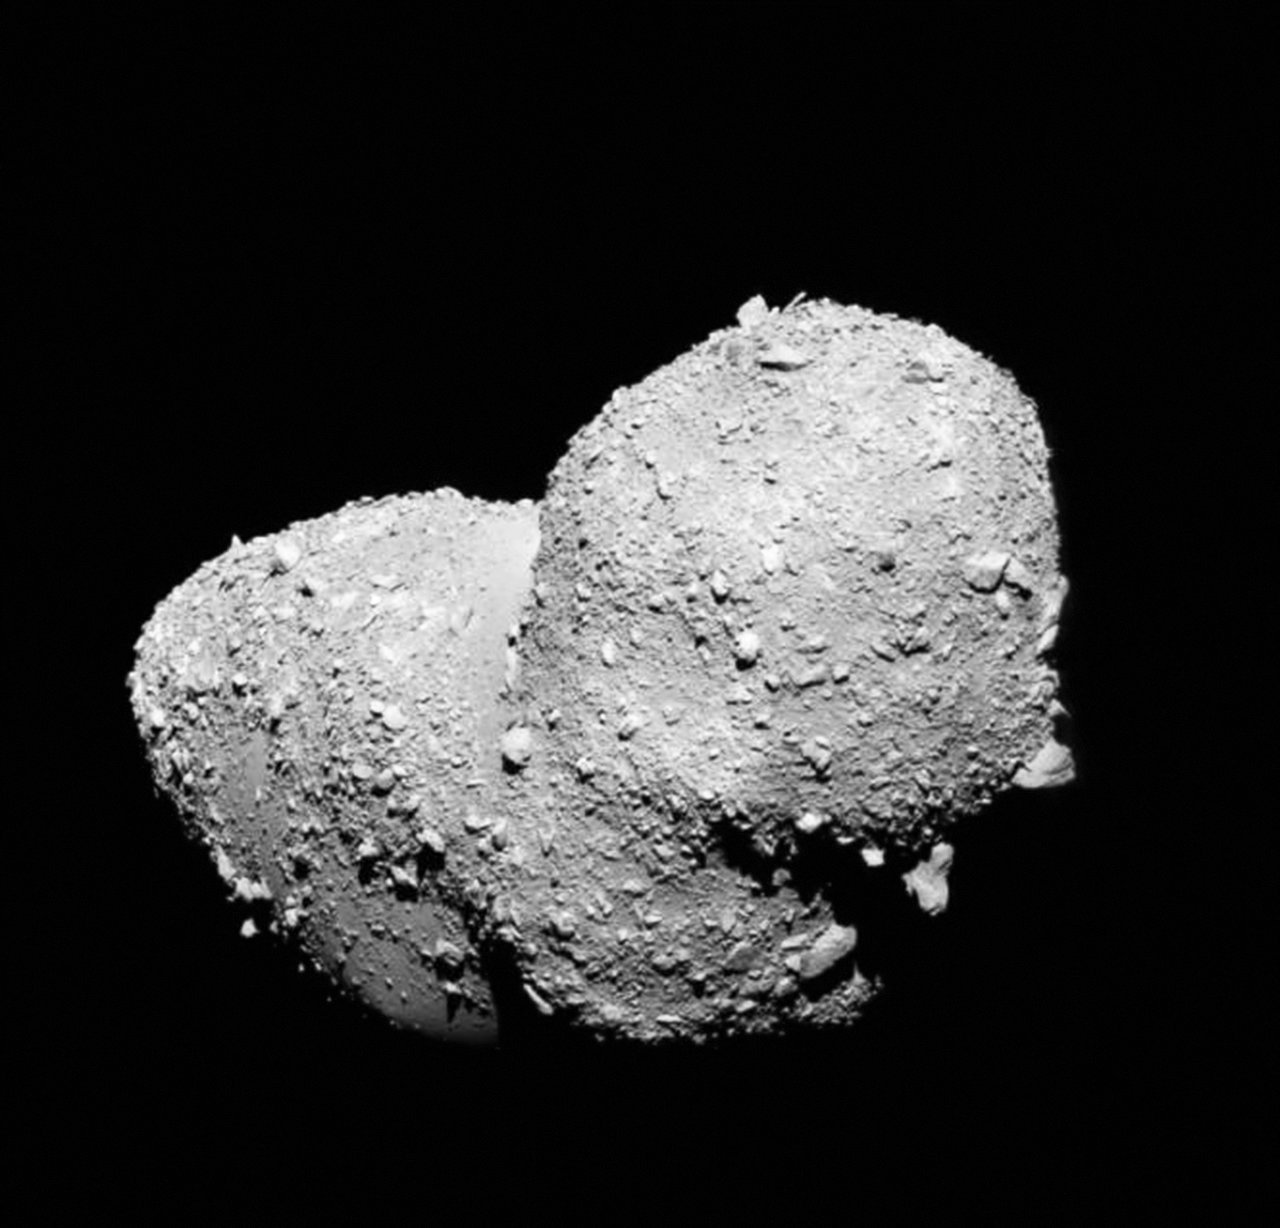
\includegraphics[height=0.3\textheight,width=0.5\textwidth, keepaspectratio]{figures/mathematical_background/eso1405b.jpg}}~
    \subcaptionbox{Comet 67/Churyumov-Gerasimenko\label{fig:67p}}{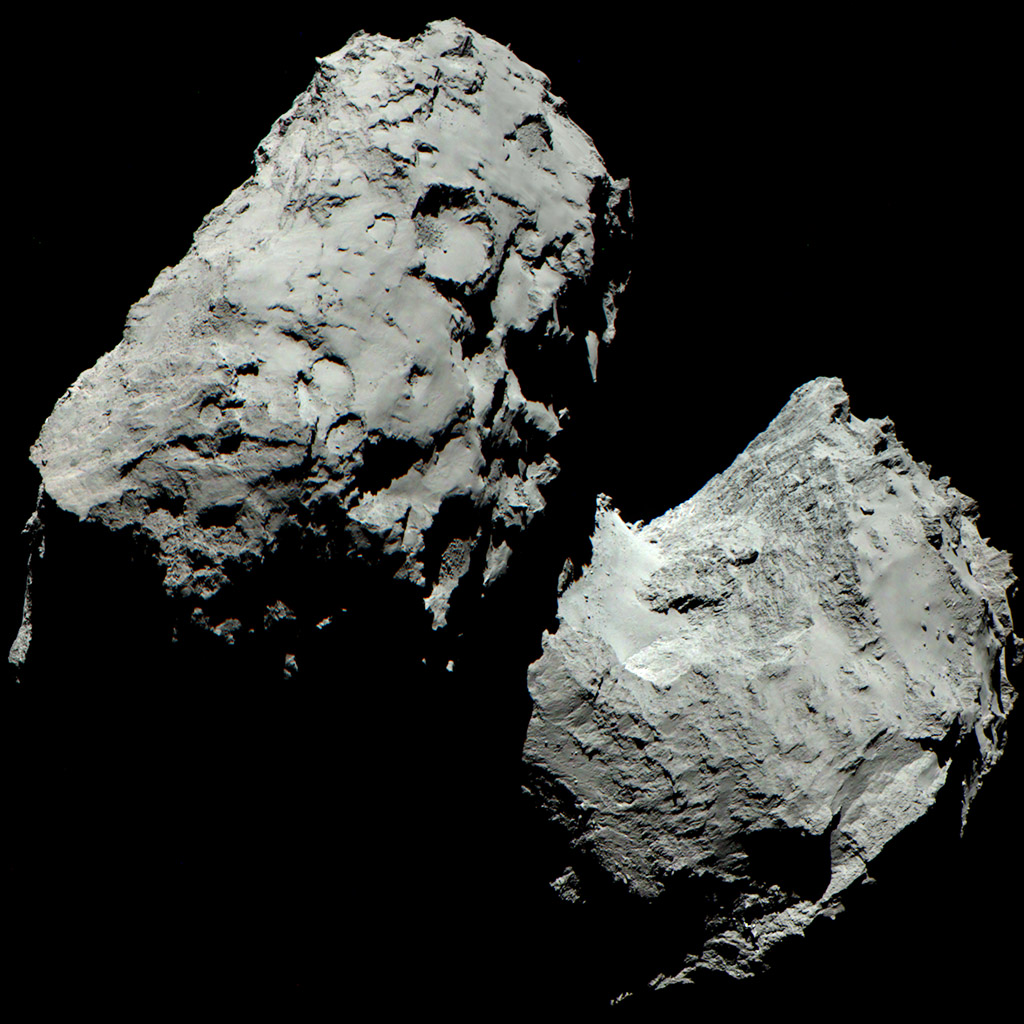
\includegraphics[height=0.3\textheight,width=0.5\textwidth,keepaspectratio]{figures/mathematical_background/comet67pcgin.jpg}}
    \caption{Examples of the non-ellipsoidal shapes of small solar system bodies. Both asteroids and comets will tend to have vastly irregular shapes due to their low mass and violent histories of impacts and collisions~\label{fig:irregular_asteroids}}
\end{figure}
The scientific community describes asteroid shape using the facet-vertex model.
This approach is an efficient representation of the more general notion of a polyhedron from geometry.
In this section, we define the notion of the polyhedron and some specifics of the format used in the astrodynamics community.


\subsection{Polyhedron Data Structures}\label{sec:polyhedron_data_structures}
While the shape of the asteroid will be represented mathematically as a polyhedron, we are still left with the issue of representing this shape in digital form. 
The eventual computational efficiency and memory consumption of the subesequent sections is heavily dependent on the underlying data structure used to represent the surface.
In this section, we review some of the basic requirements and features of any data structure.
In addition, we summarize the ones most popular in the astrodynamics community and the halfedge data structure which we use in this work.

The requirements for any surface/mesh data structure vary between applications and are designed to satisfy both topological and algorithmic requirements.
Some examples of topological considerations are the use of triangular/polygonal facets or the ability to represent manifold/non-manifold meshes.
Examples of algorithmic requirements include a consideration of the types of algorithms/processes that will make use of the data, such as visualization or operations that will modify or additional data to the various faces, edges, and vertices of the mesh.
The choice, and eventual design, of an appropriate data structure is evaluated on its ability to efficiently enable specific operations, such as distance or modification operations.
A wide variety of data structures have been developed to represent general polyhedron surfaces and can be classified as either \textit{face-based} or \textit{edge-based}.

The simplest method to represent a surface mesh is composed to storing the individual vertices which define each face of the surface.
In the specific case of a triangular mesh, this entails storing the three vertex coordinates of each face of the mesh, also called the \textit{face-set}~\cite{botsch2010}.
By assuming that the vertex coordinates are stored as double precision, or \SI{64}{\bit} values, results in \( 3 \cdot 3 \cdot 64 = \SI{576}{\bit} = \SI{72}{\byte}\) per triangular face.
% TODO Add reference to euler's formula
Equivalently, from Euler's formula, there is approximately twice as many faces as vertices, and this \textit{face-set} structure will require on average \SI{144}{\byte} per vertex.
A simple optimization is possible by reducing the redundancy in the representation.
Each vertex will duplicated as many times as the degree of the vertex.
This redundancy can be eliminated by storing a list of vertices, and to define the vertices of each face as an index/reference into this vertex list.
This results in the so called \textit{indexed face set} or \textit{shared-vertex} data structure.
In the case of triangular meshes and using double precision values, each vertex will require \(\SI{192}{\bit} = \SI{24}{\byte}\).
Vertex indices of each face can be stored using single precision, \( \SI{32}{\bit} = \SI{4}{\byte}\), values which resuts in a storage requirement of \( \SI{96}{\bit} = \SI{12}{\byte}\) per triangle.
This type of representation will therefore require on average approximately \( \SI{60}{\byte} \) per vertex, which is half the requirement of the \textit{face-set} data structure.
\begin{figure}
    \centering
    \includegraphics[width=\textwidth]{example-image-golden}
    \caption{Face based data structure look in PMP Fig2.3 or 2.4~\label{fig:face_based_data_structure}}
\end{figure}
Examples of this type of data structure include the \gls{stl}, \gls{obj}, and \gls{off} file formats.

While conceptually simple the face based data structure has several critical drawbacks.
It is difficult to determine the connectivity of individual vertices or faces of the mesh, which makes it ill-suited for most algorithms.
The vast of majority of computational geometry algorithms will require as a minimum~\cite{botsch2010}:
\begin{itemize}
    \item Access to individual vertices, edges and faces, as well as random access to any element.
    \item Enumeration of the edges of a single face.
    \item Access to the adjacent faces of an edge which enables access to the neighboring faces.
    \item Given an edge one must determine the two vertices which define the endpoints.
    \item Given a vertex one must determine all neighboring faces.
\end{itemize}
As a result, any application making use a face based data structure will need to store additional connectivity information in a seperate data structure.

In contrast to face-based structures, edge-based data structures store the connectivity information in the edges or halfedges~\cite{botsch2010,orourke1998,berg2008}.
By splitting each unorientated edge into two orientated halfedges, the halfedge data structure, or also known as the doubly-connected edge list, provides an efficient data structure for mesh based operations.
Each halfedge is ordered in a clockwise fashion around each face, typically such that the face normal is orientated outwards from the mesh.
In addition, each halfedge will also store a reference to:
\begin{itemize}
    \item The vertex it points to, or its target,
    \item its adjacent face,
    \item the next halfedge of the face in a counterclock wise direction,
    \item the previous halfedge of the face
    \item the opposite or incident halfedge.
\end{itemize}
In addition, each face stores the reference to one of its halfedges, while each vertex stores an outgoing halfedge. 
The halfedge data structure will require more memory in contrast to face based approaches it offers several advantages which make it ideal for computational geometry operations.

\subsubsection{Halfedge Data Structure}\label{sec:halfedge_data_structure}
A halfedge data structure allows us to iterate through all elements, vertices, edge, halfedge, or face, in a simple manner.
In addition, the halfge edge data structure can store arbitrary polygon meshes.
Furthermore, additional data can be attached to the elements as each is store explicitly.
Finally, the halfedge data structure allows for simple manipulation and modification of the underlying mesh, enabling operations such as mesh subdivision or simplification.
There are a number of publicly avaiable implementations of the halfedge data structure~\cite{cgalproject2018,botsch2002}.
We utilize the \texttt{Surface\_mesh} data structure implemented within the Computational Geometry Algorithms Library~\cite{sieger2011}.
This provides a well defined and highly optimzed data structure for the representation of the polyhedron shape of the asteroid.
Furthermore, the ability to incorporate additional properties enables us to efficently compute the polyheron potential model.
\begin{figure}
    \centering
    \includegraphics[width=\textwidth]{example-image-golden}
    \caption{Halfedge data structure look in PMP Fig3.4~\label{fig:halfedge_data_structure}}
\end{figure}

\begin{figure}
    \centering
    \includegraphics[width=\textwidth]{example-image-golden}
    \caption{Iterating over 1 ring of a vertex}
\end{figure}
% TODO Describe the halfedge data structure and Surface_mesh in more detail

\subsubsection{Wavefront OBJ files}
The OBJ format is a geometry definition file format used for a variety of computer modeling applications, and is regularly used by the asteroid community~\cite{neese2004}.
The basic format of the file is an ASCII file where the first \( N_v\) lines begin with \texttt{v} and define the three components of a vertex in the body fixed reference frame.
The following \( N_f\) lines begin with \texttt{f} and define the three indices of the vertices that make up the face.
The numbering of the vertices is implicitly defined by the order listed in the file, i.e. the vertices are defined from \( 1 \) to \( N_v\).
There are two main assumptions used by the asteroid community.
First, each face is triangular and second, the vertices are numbered in a counterclockwise fashion about each face.
This allows the outward facing normal to each face to be uniquely defined without any additional data.

This polyhedron model, captured using the OBJ format, allows for a much larger class of potential object shapes. 
The accuracy of the shape model can be arbitrarily improved by incorporating additional vertices and faces, which increase the resolution of the model in regions of high complexity.
The polyhedron model can capture arbitrary depressions, ridges, or holes through the asteroid.
Small bodies typically lack sufficient mass to create regular, spherical shapes, and exhibit a large variety in resulting shapes such as the examples shown in~\cref{fig:asteroid_shape}.
\begin{figure}
    \centering
    \subcaptionbox{4769 Castalia\label{fig:castalia}}{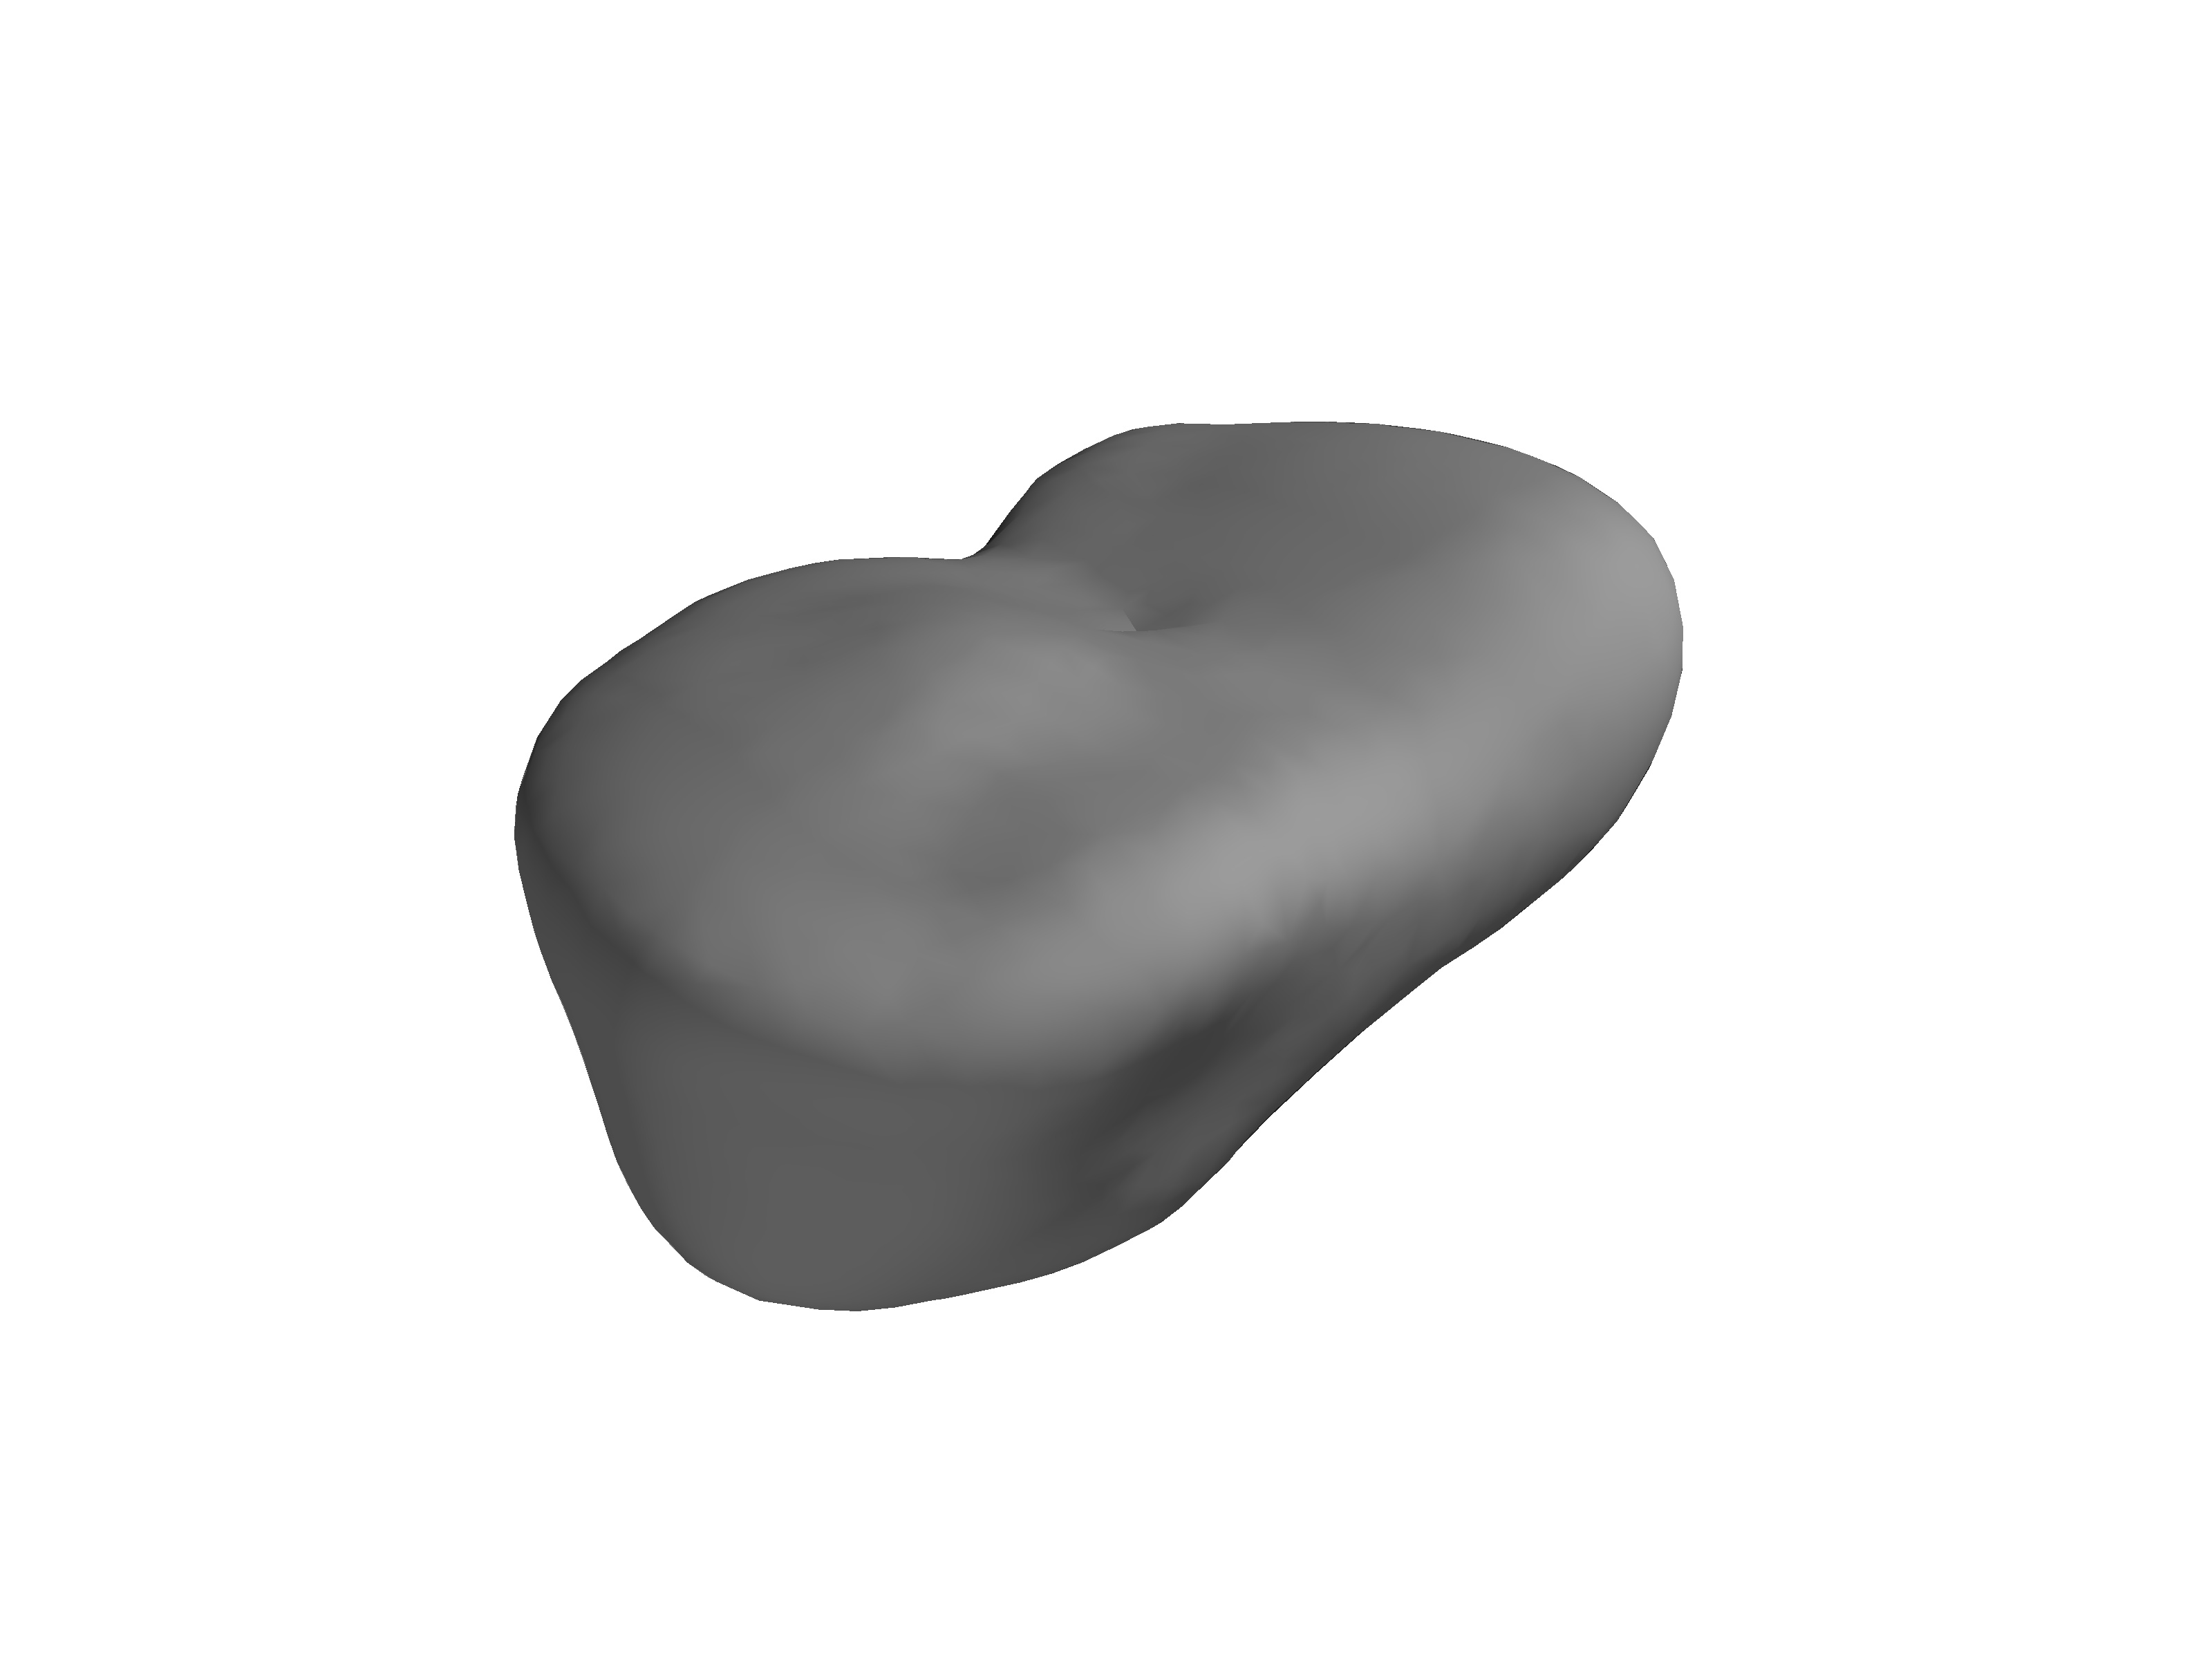
\includegraphics[width=0.33\textwidth]{figures/mathematical_background/castalia_isometric.jpg}}~
    \subcaptionbox{Geographus\label{fig:geographus}}{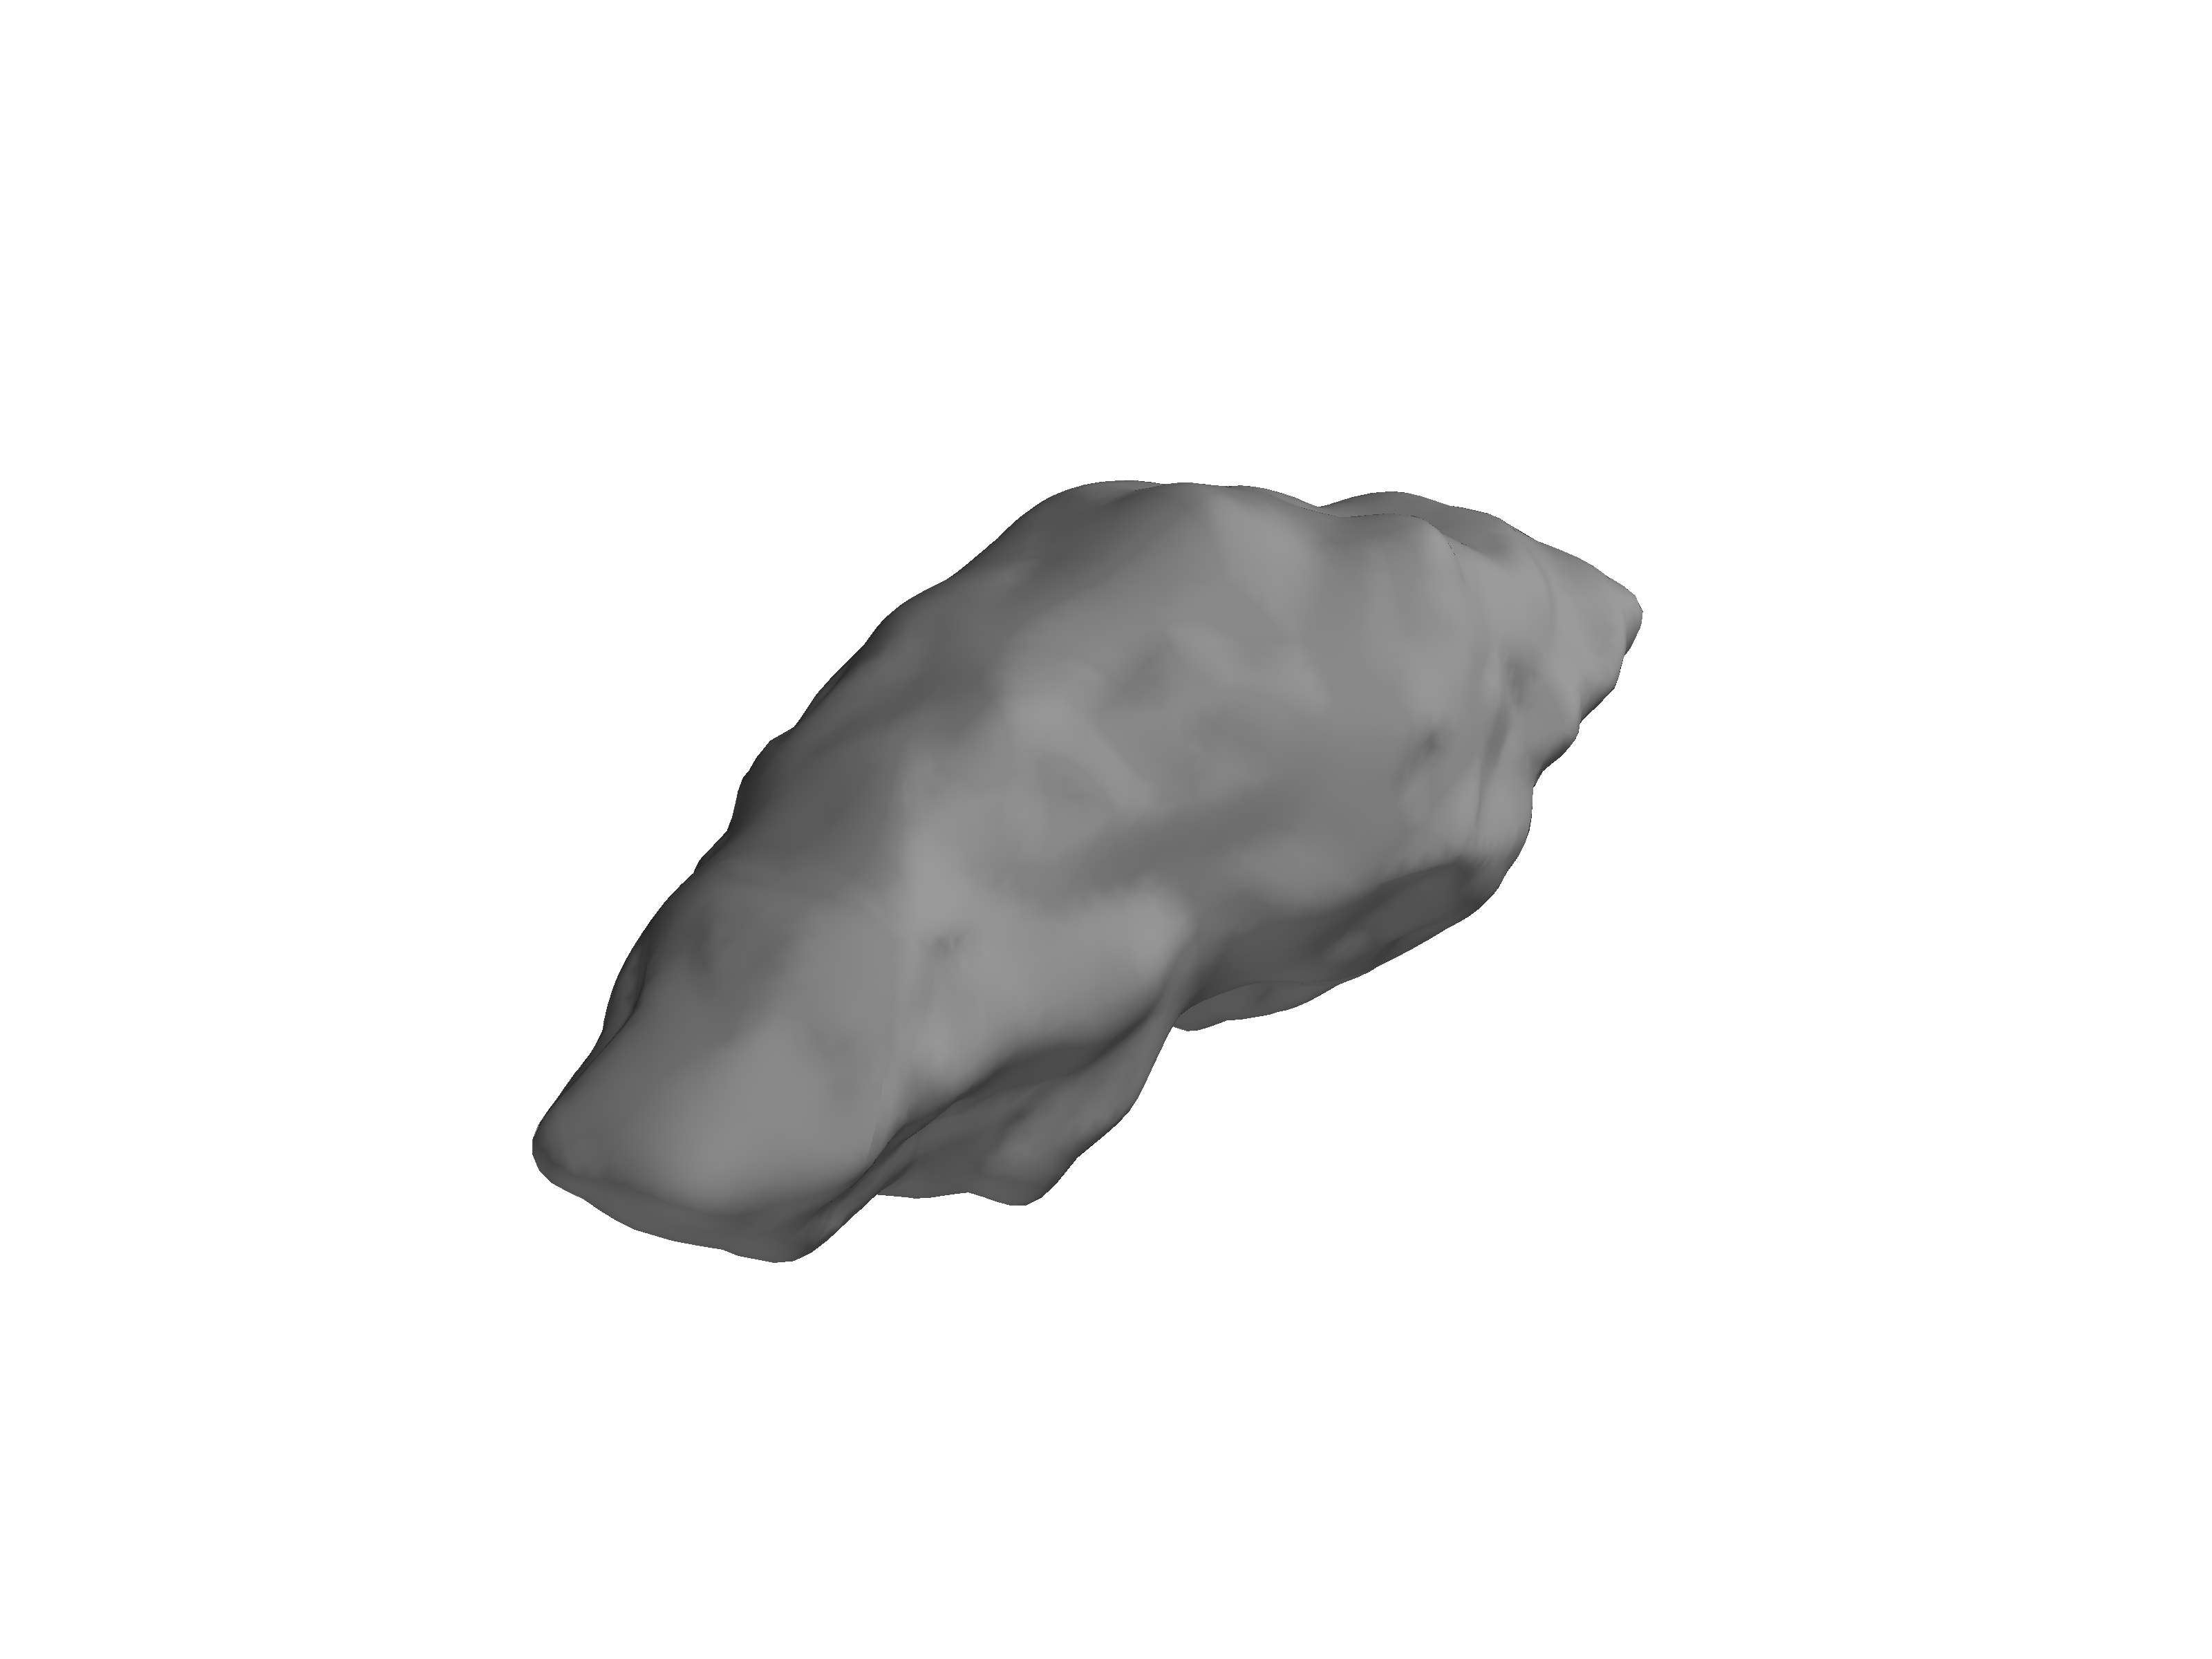
\includegraphics[width=0.33\textwidth]{figures/mathematical_background/geographus_isometric.jpg}}~
    \subcaptionbox{Golevka\label{fig:golevka}}{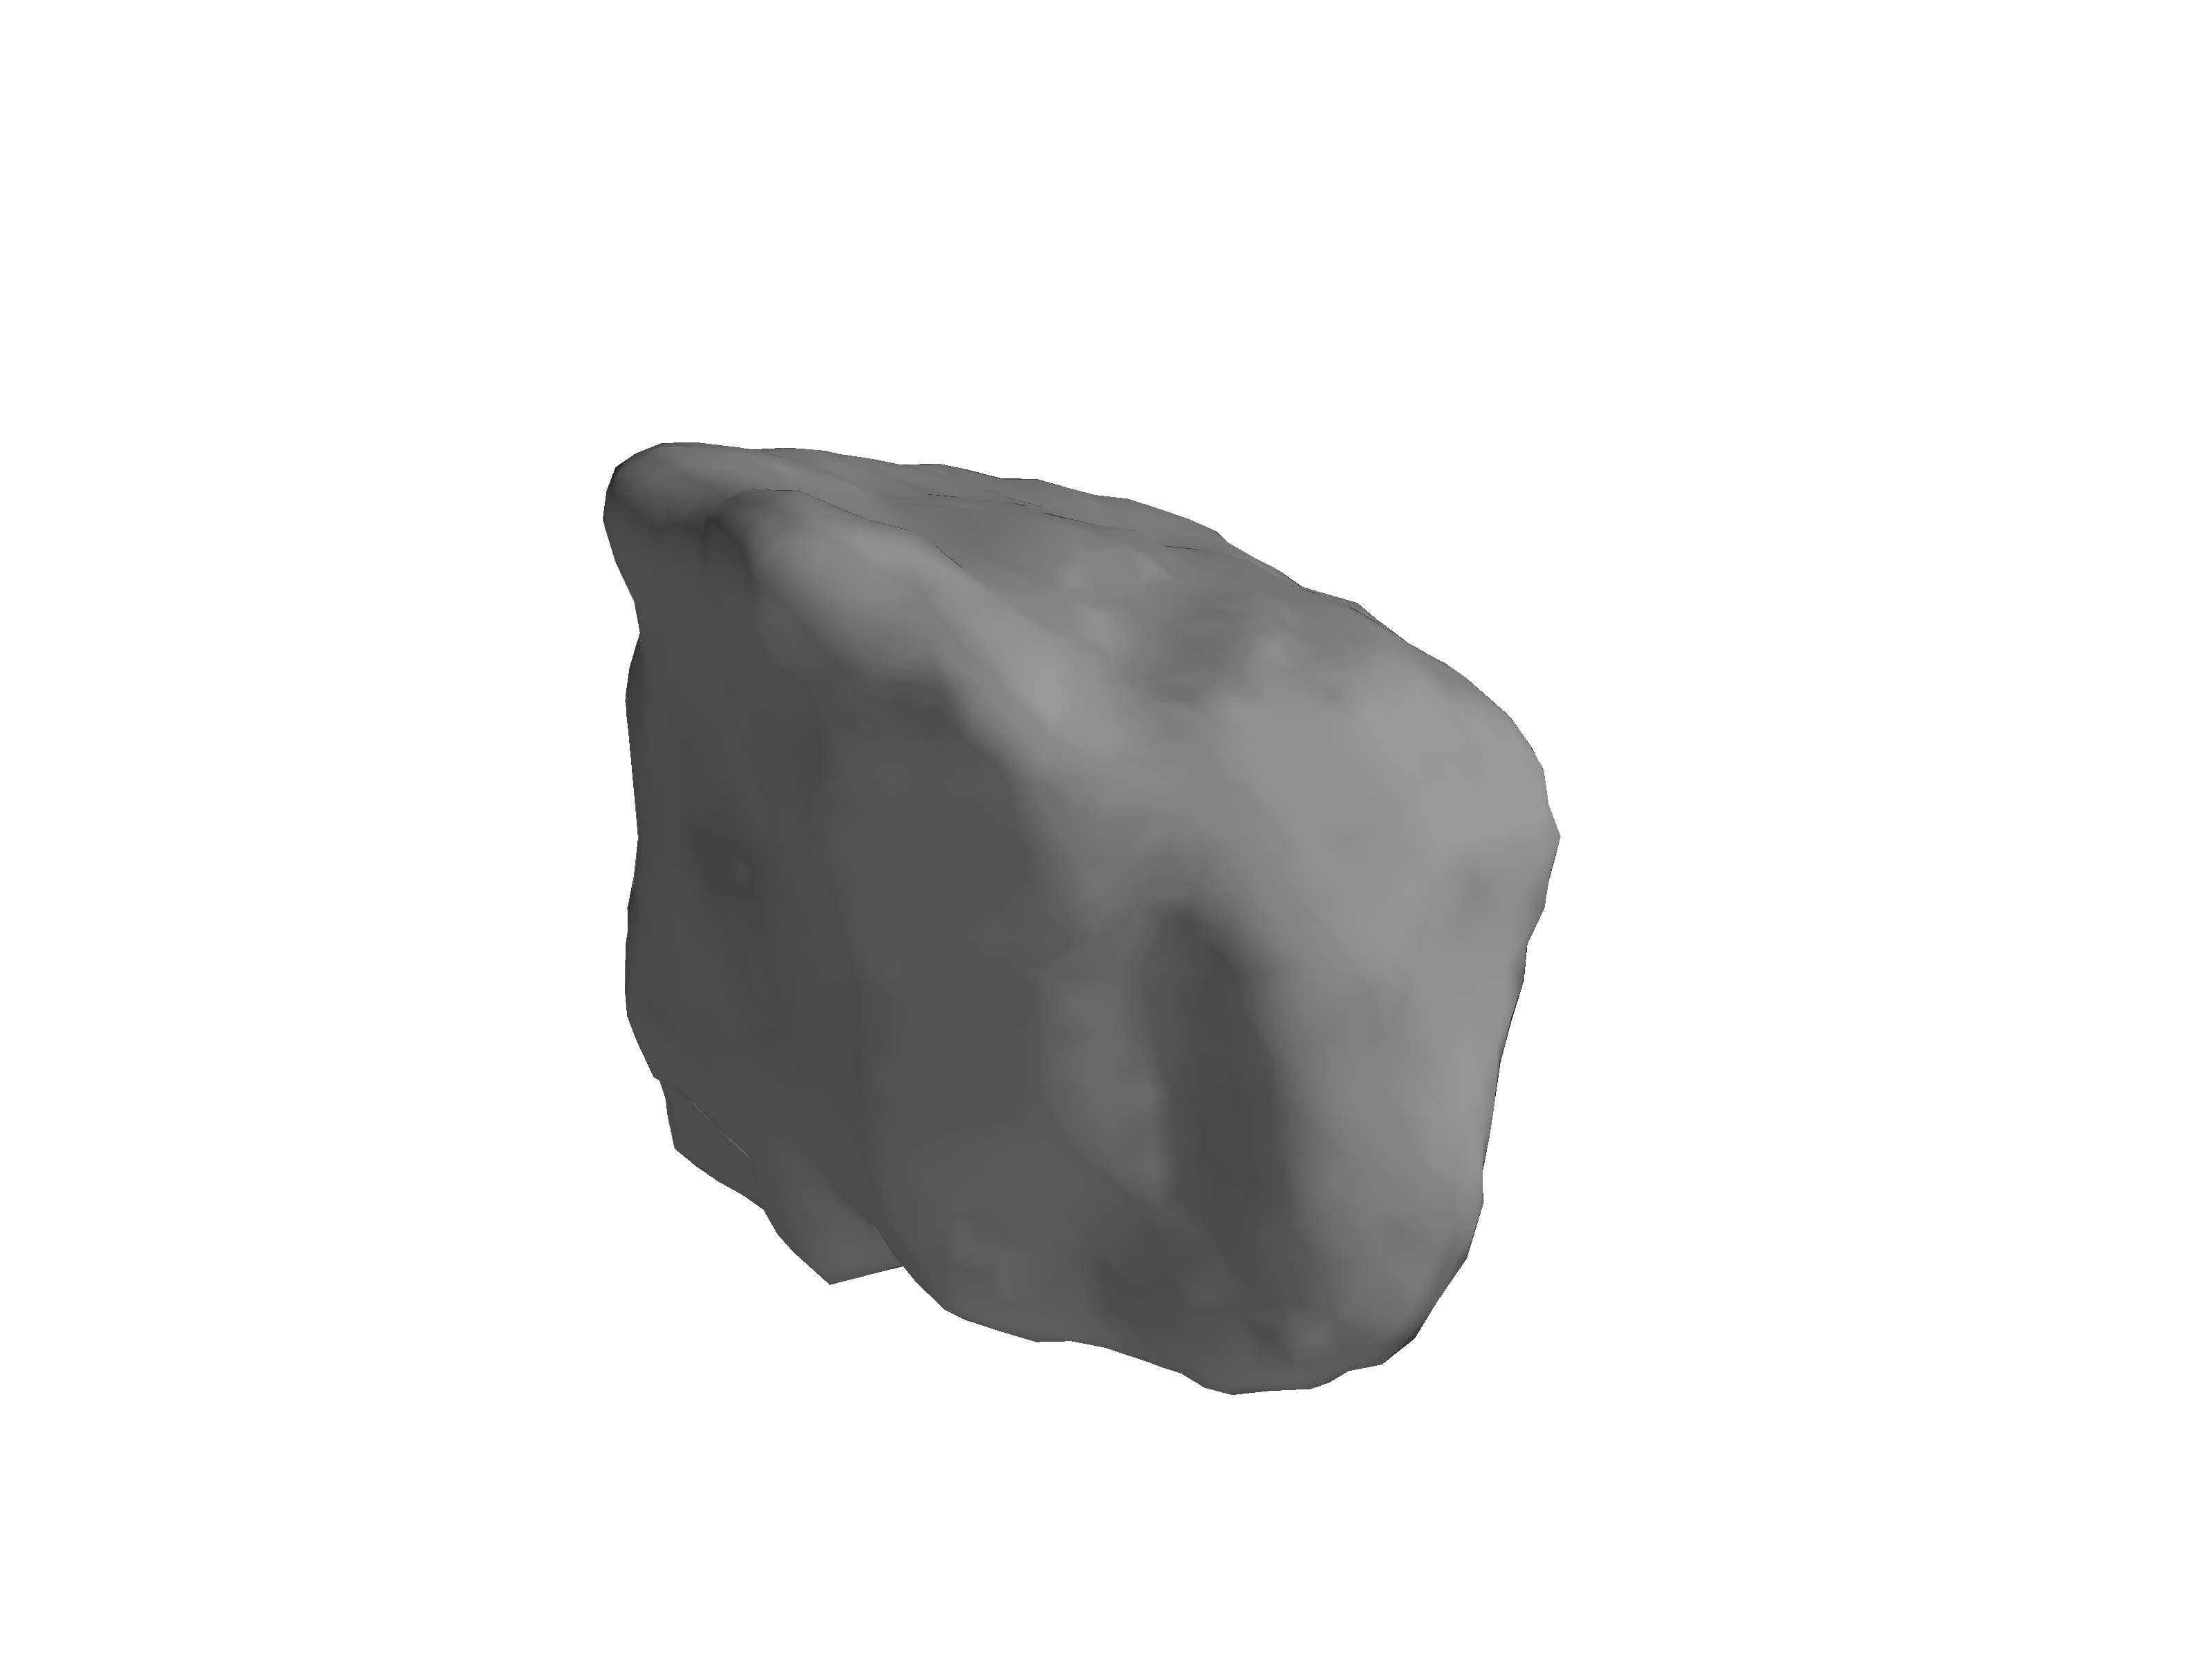
\includegraphics[width=0.33\textwidth]{figures/mathematical_background/golevka_isometric.jpg}}
    \caption{Polyhedron Shape Models for several asteroids~\label{fig:asteroid_shape}}
\end{figure}
Polyhedron shape models are available for several asteroids~\cite{neese2004,gaskell2008b}.
The quality and resolution is dependent on the measurement available of the body.
\Cref{fig:itokawa_radar} shows a polyhedron model of asteroid 25143 Itokawa based on ground radar measurements~\cite{neese2004}.
This model is composed of \num{6098} vertices and \num{12192} faces and captures the general ellipsoidal shape of the asteroid.
However, ground based measurements are unable to provide the resolution required to capture the fine details or even the asymmetry of asteroid Itokawa.
In contrast,~\cref{fig:itokawa_insitu} shows the model derived from in-situ measurements from optical sensor of the Hyabusa spacecraft~\cite{gaskell2008a}.
It is composed of \num{1579014} vertices and \num{3145728} faces and is able to capture small surface features such as boulders.
\begin{figure}
    \centering
    \subcaptionbox{25143 Itokawa Radar Model\label{fig:itokawa_radar}}{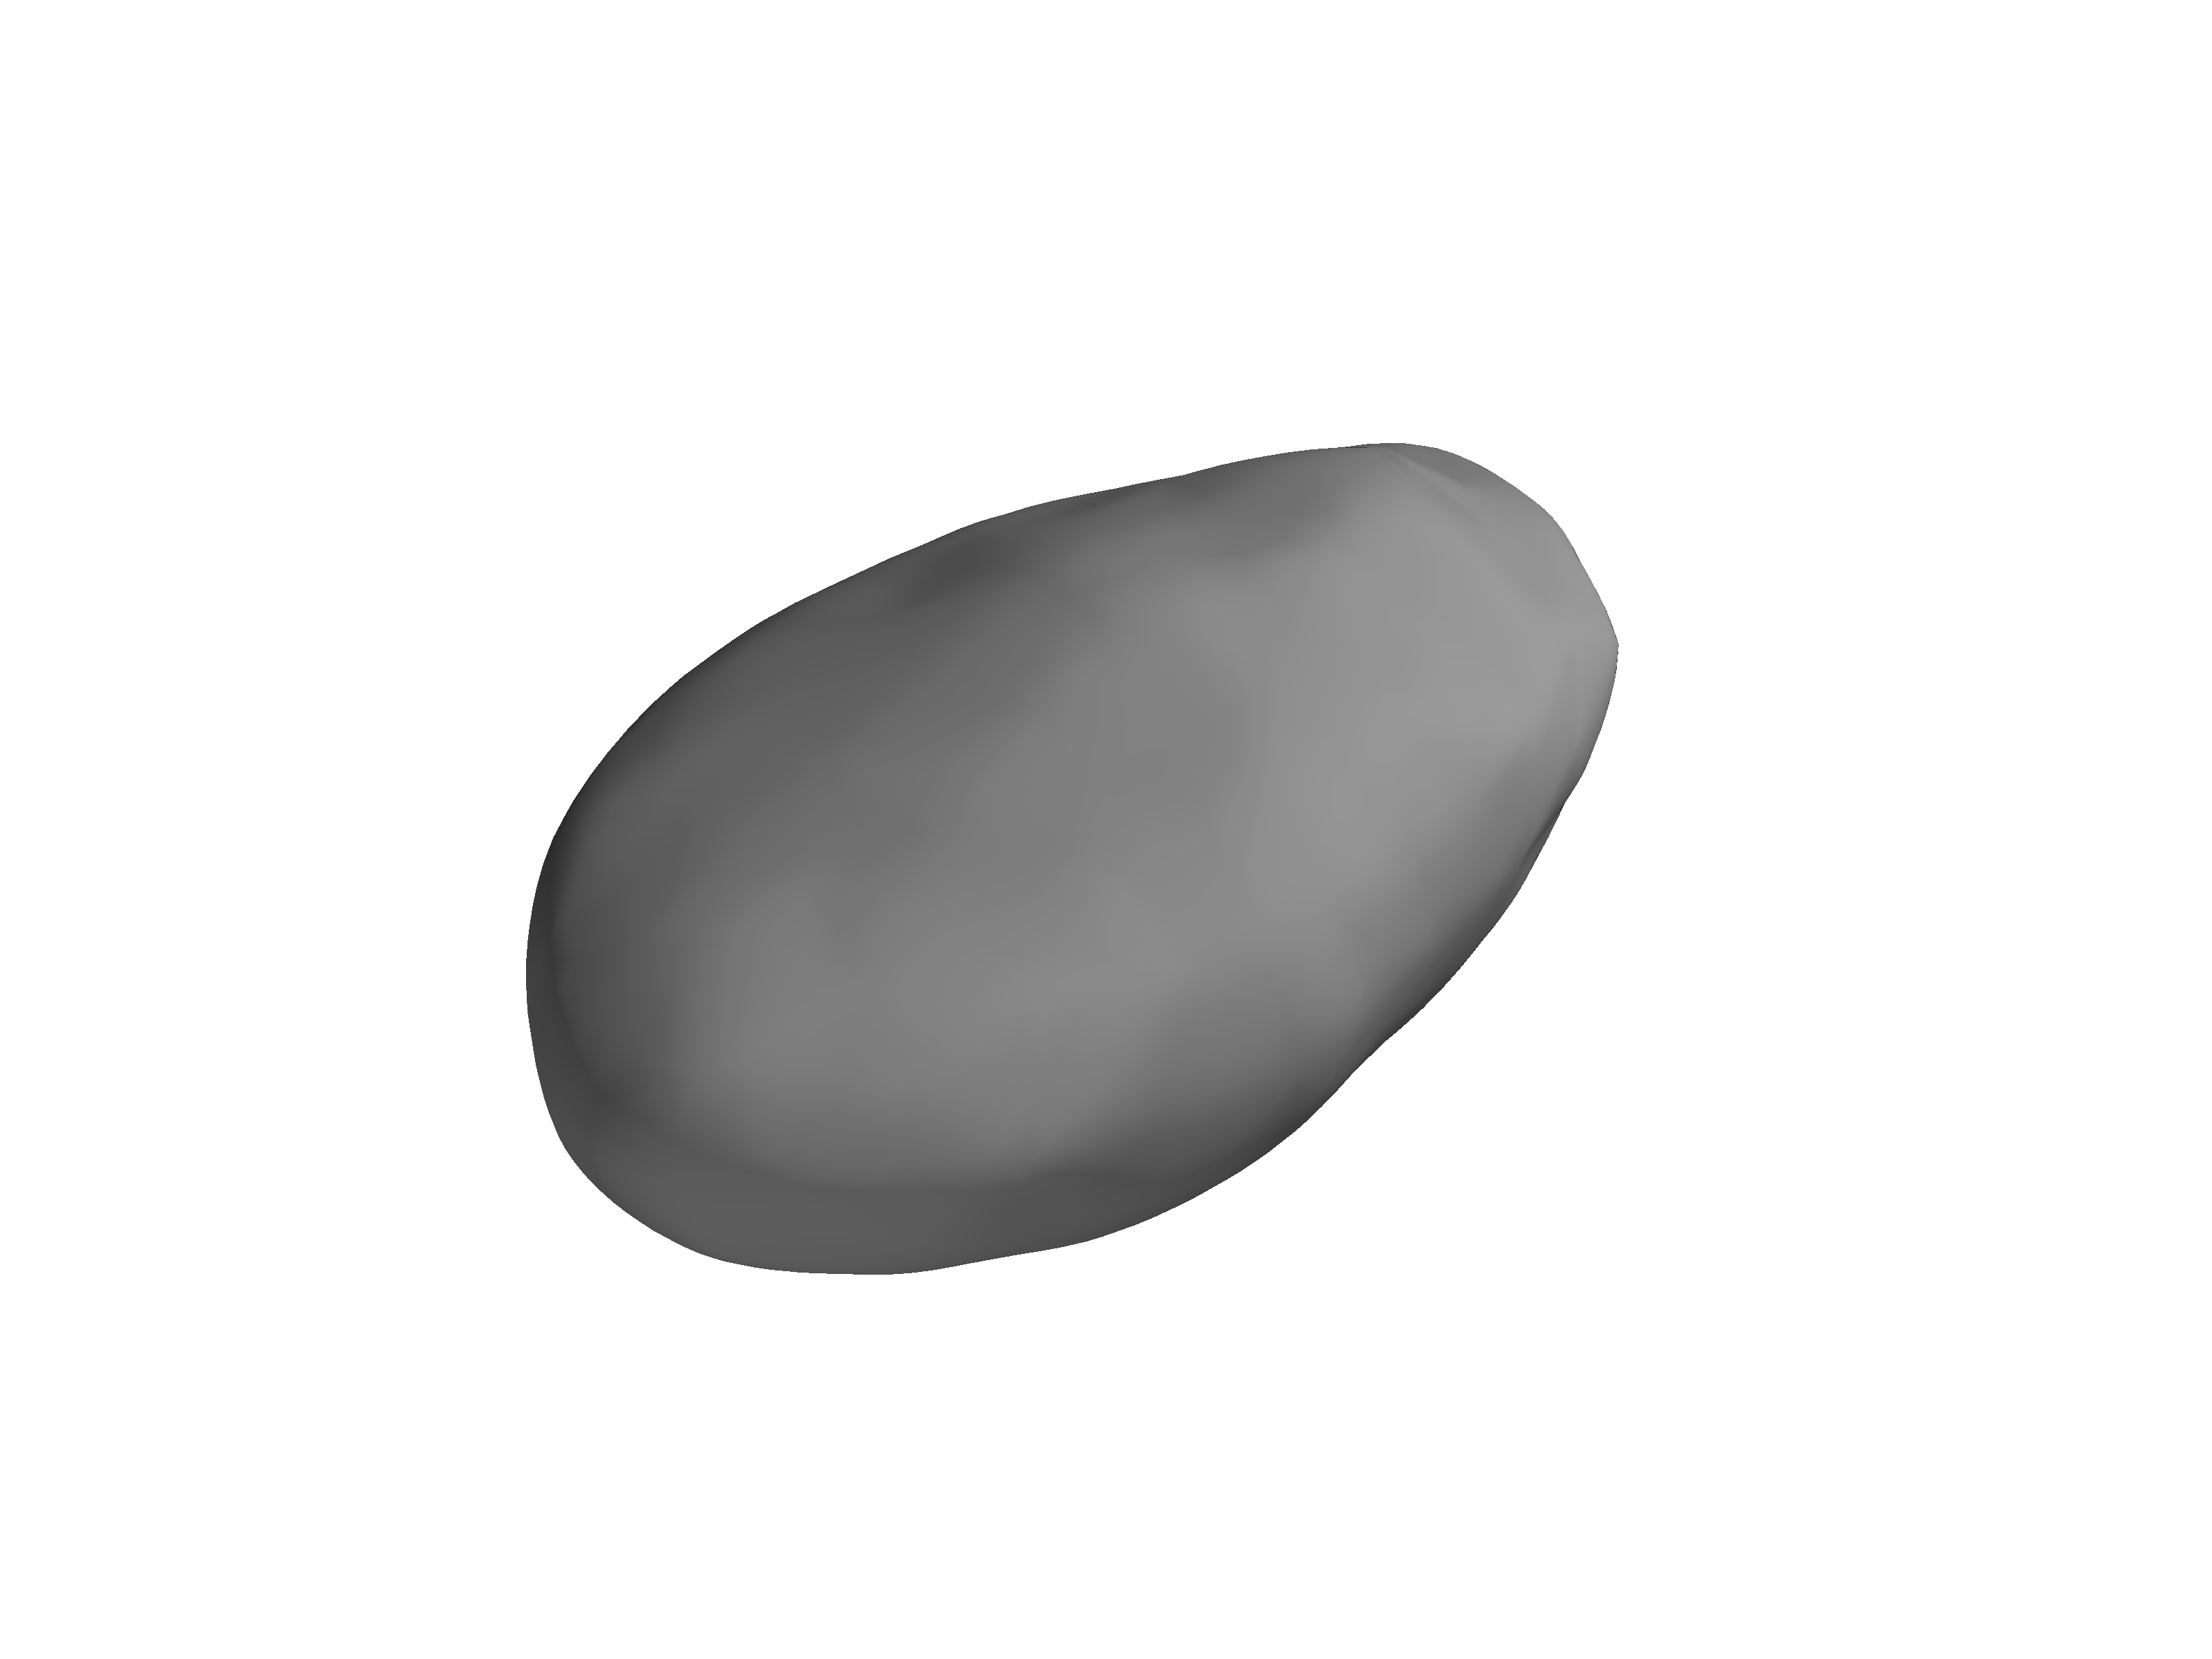
\includegraphics[width=0.5\textwidth]{figures/mathematical_background/itokawa_radar_isometric.jpg}}~
    \subcaptionbox{25143 Itokawa In-Situ Model\label{fig:itokawa_insitu}}{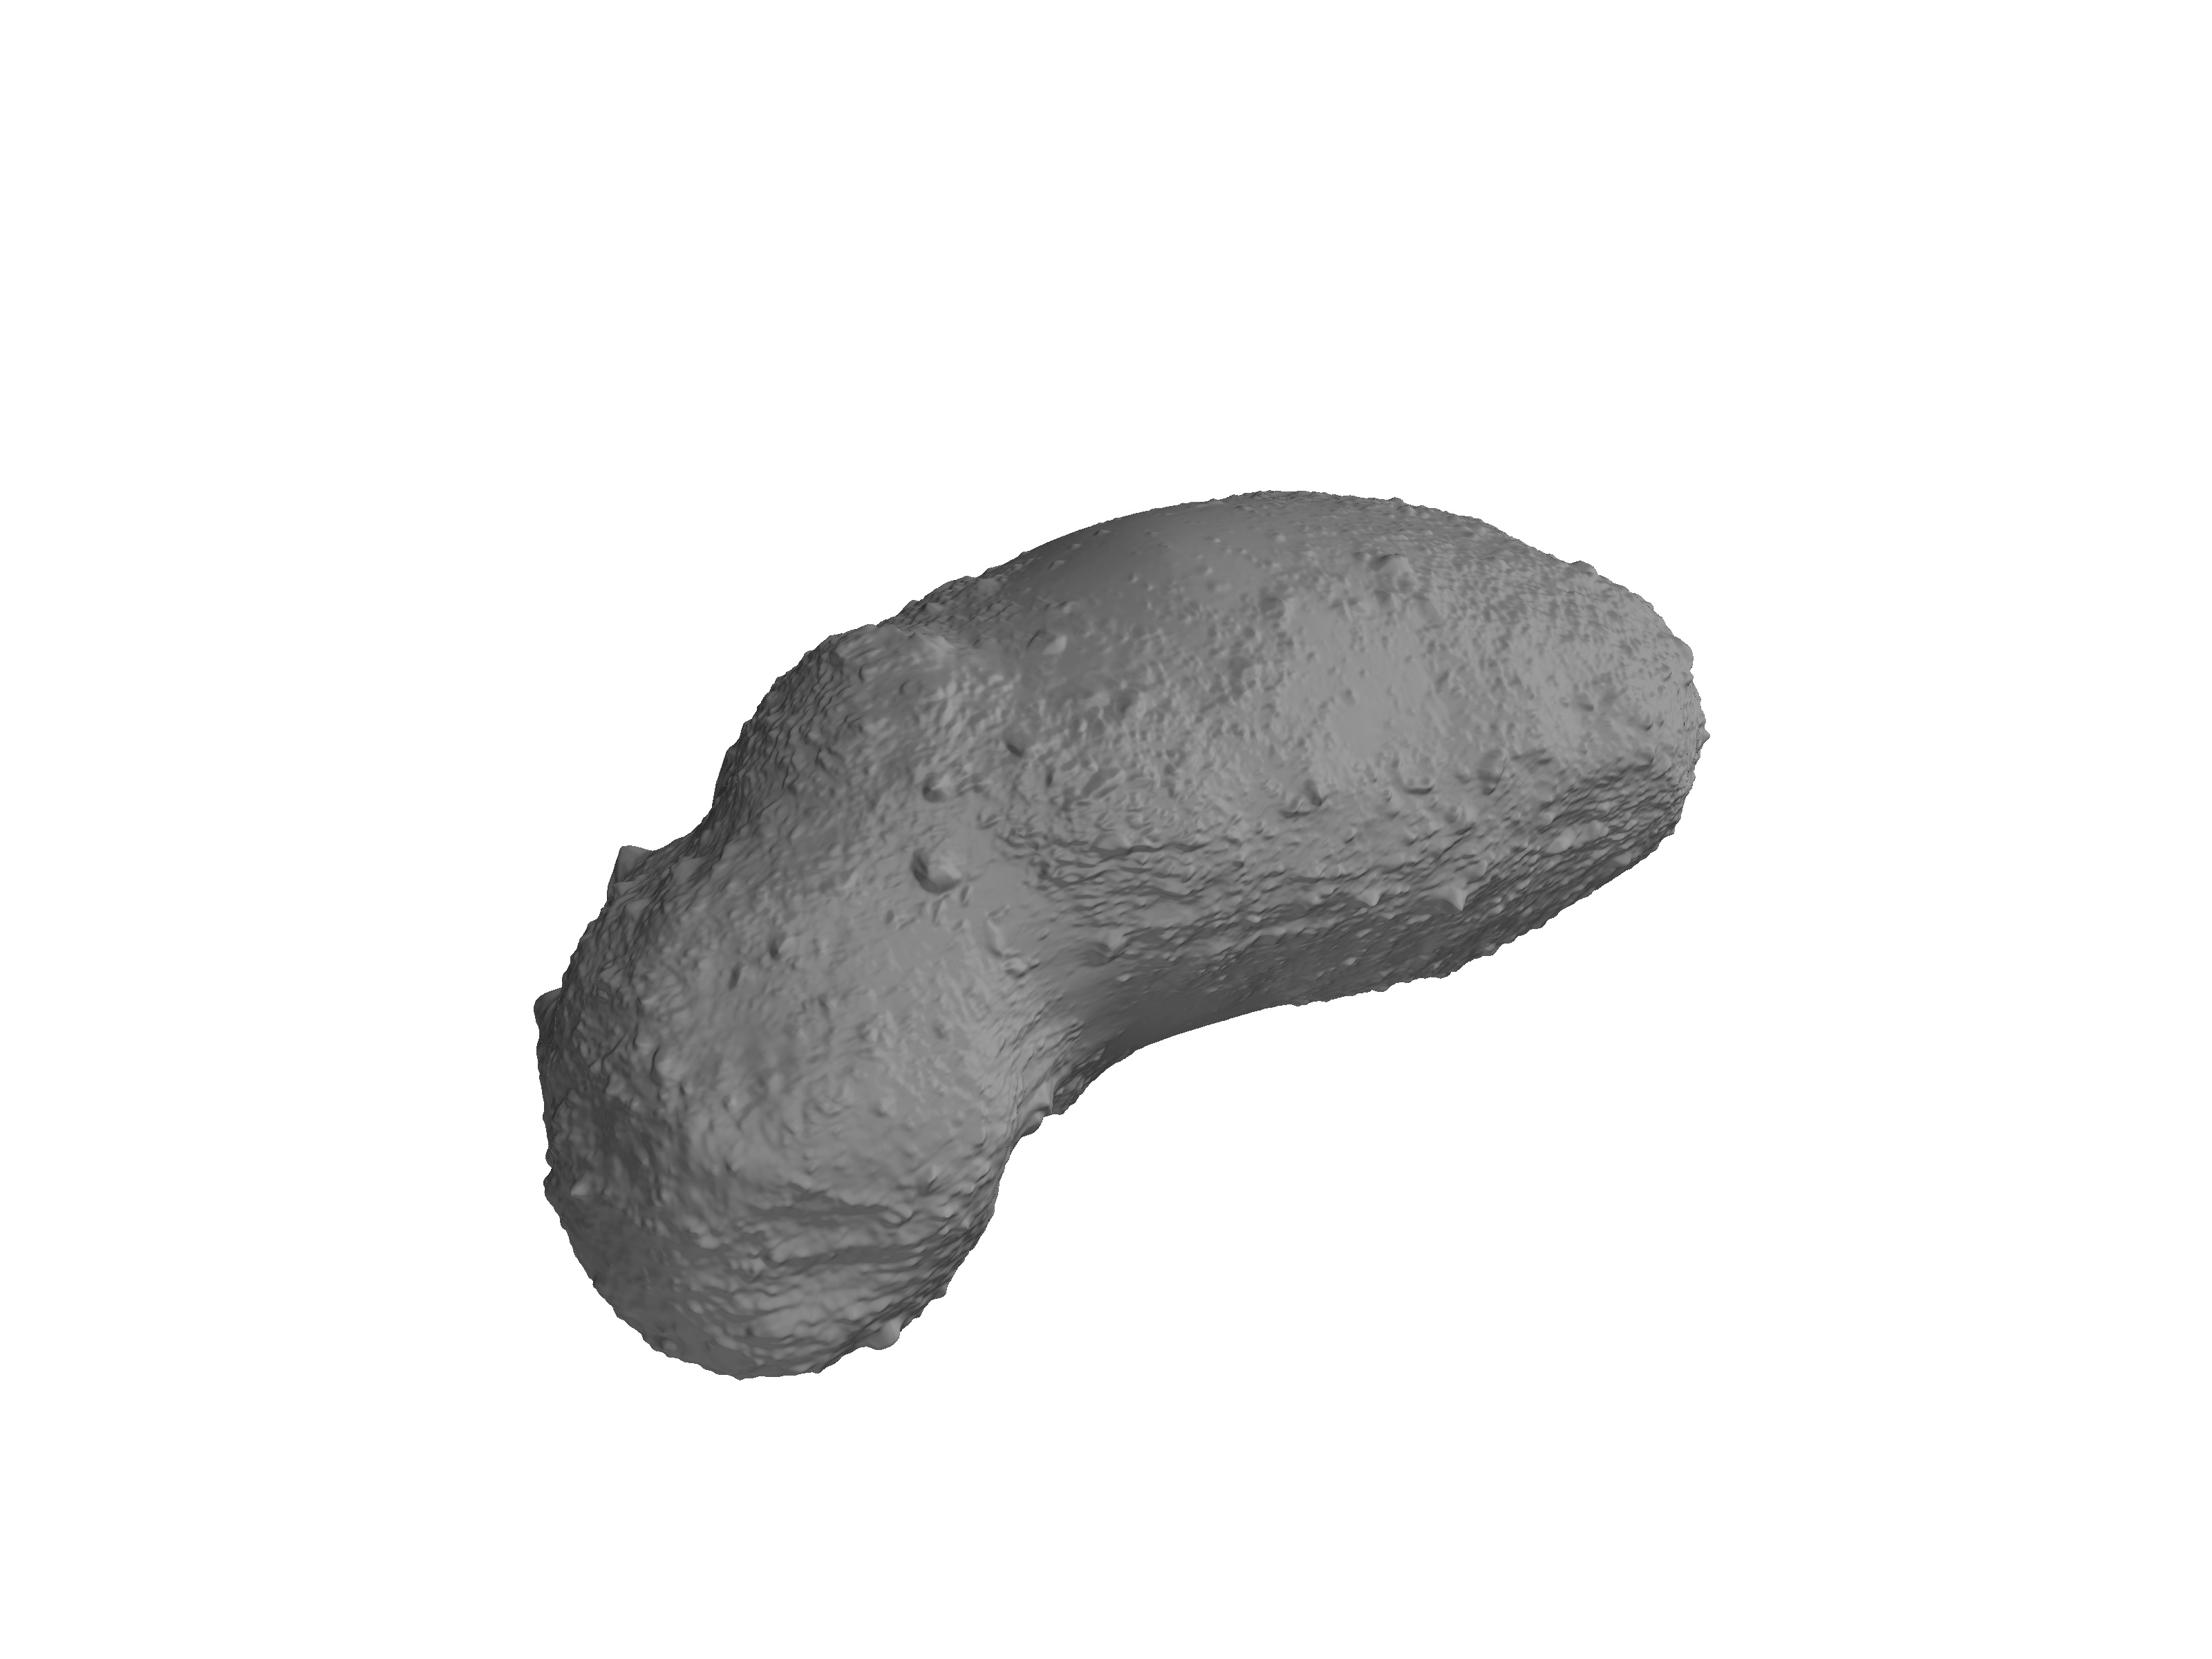
\includegraphics[width=0.5\textwidth]{figures/mathematical_background/itokawa_isometric.jpg}}
    \caption[Comparison of Radar and In-situ Itokawa models]{Comparision of polyhedron models of 25143 Itokawa based on ground based radar or in-situ measurements.
        The ground based model can capture the rough ellipsoidal shape but does not capture fine surface details.}
\end{figure}
From this simple example, it is clear that prior to the arrival of a spacecraft the shape and surface knowledge of an asteroid is limited.
